\documentclass[a4,openany,portrait,tikz]{article}
%\documentclass[a4,openany,landscape,tikz]{article}
%\documentclass[11pt,a5,landscape,openany]{article}
\usepackage{xcolor}
\usepackage{makeidx}
\usepackage{geometry}       
\usepackage[chorded]{songs} 
\usepackage[colorlinks=true, pdfstartview=FitV, linkcolor=blue, citecolor=blue, urlcolor=blue]{hyperref} 
%\usepackage{fancyhdr}
%\usepackage{abc}
%\usepackage{lilypond}
%\usepackage[parfill]{parskip}  
\usepackage{graphicx}
\usepackage{wrapfig}
\usepackage{qrcode}
%\usepackage{amssymb}
%\usepackage{epstopdf}
%\DeclareGraphicsRule{.tif}{png}{.png}{`convert #1 `dirname #1`/`basename #1 .tif`.png}
%\usepackage{xpatch}

\usepackage{tikz}
\usetikzlibrary{decorations.text}


% this was used when it was landscape: 
%\setlength{\topmargin}{-0.5cm}
%\setlength{\headheight}{0cm}
%\setlength{\headsep}{-0.5cm}
%\setlength{\textheight}{18cm}
%\setlength{\textwidth}{24cm}
%\setlength{\oddsidemargin}{-0.5cm}
%\setlength{\evensidemargin}{-0.5cm}	
%\setlength{\parindent}{0.25cm}

\setlength{\topmargin}{-0.5cm}
\setlength{\headheight}{0cm}
\setlength{\headsep}{-0.5cm}
\setlength{\textheight}{25cm}
\setlength{\textwidth}{18cm}
\setlength{\oddsidemargin}{0cm}
\setlength{\evensidemargin}{0cm}
\setlength{\parindent}{0.25cm}


%never used? \setlength{\parskip}{0.25cm}


\songpos{2}

%\pagestyle{fancy}
%\fancyhf{}
%\lfoot{%
%	\begin{minipage}{\textwidth}
%	\parbox{0.46\linewidth}{Some text to go in the footer Some text to go in the footer}\hfill
%	\parbox{0.70\linewidth}{\includegraphics[width=0.2\linewidth]{KK/KuylKamp_vierkantje_logo}}\hfill
%	\parbox{0.60\linewidth}{\raggedleft
\includegraphics[width=0.2\linewidth]{KK/KuylKamp_naam}}\hfill
%	\parbox{0.02\linewidth}{\raggedleft \thepage}%
%	\end{minipage}
%}

\renewcommand\printchord[1]{{\color{red!70!black}#1}}

\renewcommand{\songchapter}{\subsection}
\renewcommand{\songsection}{\subsection}

\newcommand{\U}{\Uparrow}
\newcommand{\D}{\Downarrow}

\pagenumbering{gobble}

% ------------------- Title and Author -----------------------------
\title{AMeeSpeel KuylKampVuur Songbook 2016}

\author{gathered by Grobozeak-KKVO}
\newindex{titleidx}{titleidx}
\indexsongsas{titleidx}{\thepage}
%\newauthorindex{authidx}{authidx}

%\frontmatter

\begin{document}
%\songcolumns{2}

\maketitle 

%\qrcode[hyperlink]{https://www.kuylkamp.nl}

%\parbox{0.70\linewidth}{\includegraphics[width=0.2\linewidth]{KK/KuylKamp_vierkantje_logo}}\hfill

 
\begin{wrapfigure}{l}{0.20\textwidth}
\qrcode[hyperlink]{https://github.com/coentjo/songbooks/releases}

%\url{https://github.com/coentjo/songbooks/releases}. 
\end{wrapfigure}


Bij een aantal nummers is aangegeven op welke positie de capo moet staan om met het origineel mee te kunnen spelen (als je het bijvoorbeeld op youtube opzoekt). Op het KuylKamp zullen we zoveel mogelijk \emph{zonder} spelen.  

Dit songbook is ook te vinden op internet, verstopt achter de URL \url{https://github.com/coentjo/songbooks/releases}. 

Op die internetpagina staan ook een aantal links naar opnamen van een aantal nummers zoals ze ook in de map staan.  
Natuurlijk heb je een gestemde gitaar nodig. Als je geen stemmer hebt kun je je mobiel gebruiken met een app: Zoek in de app store van je keuze op `\emph{Guitar Tuner}'. Zelf heb ik goeie ervaringen met `PitchLab Guitar Tuner' onder Android. 

Na het KuylKamp ben ik weer wat nummers aan het toevoegen, niet allemaal geschikt als kampvuur, maar dat zoeken we volgend jaar vlak voor het KuylKamp wel weer uit... Check af en toe eens voor updates... 

Fouten, wijzigingen of andere tips? Geef ze door via email:   \href{mailto:coentjo@gmail.com}{coentjo@gmail.com} 

\includegraphics[width=0.2\linewidth]{KK/guitar-image-7} 


\begin{wrapfigure}{l}{0.25\textwidth}
\includegraphics[width=0.3\linewidth]{KK/KuylKamp_vierkantje_logo} 
\end{wrapfigure}


\begin{tikzpicture}[mypostaction/.style 2 args={
                         decoration={
                              text align={
                                    left indent=#1},
                                    text along path, 
                                    text={#2}
                                    },
                           decorate
                        }
                    ]
  \coordinate (specRoot) at (-10,0);
  \coordinate (testTreeRoot) at (0,0);
  \draw[-latex, blue!20!white, line width=5ex]  (specRoot) to[in=135,out=45] (testTreeRoot);

  \path [postaction={mypostaction={1cm}{Sla snel de bladzijde om}},
         postaction={mypostaction={1cm}{en begin met spelen!},
         /pgf/decoration/raise=-3mm}]
    (specRoot) to [in=120,out=45] (testTreeRoot);
\end{tikzpicture}

%\url{https://github.com/coentjo/songbooks/releases/download/v0.1/Amy_Green.Day.mp3}
%\qrcode{https://github.com/coentjo/songbooks/releases/download/v0.1/Amy_Green.Day.mp3}

\showindex[1]{Title index}{titleidx}


%\tableofcontents 
%\showindex{Al hun liedjes}{titleidx}

%\showindex[2]{Nummers}{titleidx}
%\showindex[2]{artiesten}{authidx}


%\begin{abc}[name=c-dur]
%X: 1 % start of header
%K: C % scale: C major
%"Text"C4 G4 | (3FED c4 G2 |
%\end{abc}
\newpage

\begin{songs}{titleidx} %,authidx}
\songcolumns{1}

	
\renewcommand{\thesongnum}{A}
	% Activate the following line by filling in the right side. If for example the name of the root file is Main.tex, write
% "...root = Main.tex" if the chapter file is in the same directory, and "...root = ../Main.tex" if the chapter is in a subdirectory.
 
%!TEX root = ../boktor.tex 

\beginsong{Act Naturally (in G)}[by=Beatles]


%{\nolyrics Intro: \[E] \[G] \[A]}


\beginverse
They're gonna put me in the movies
They're gonna make a big star out of me
We'll make a film about a man that's sad and lonely
And all I gotta do is act naturally
\endverse

\beginverse
Well, I'll bet you I'm gonna be a big star
Might win an Oscar you can never tell
The movies gonna make me a big star
Cos I can play the part so well
\endverse

\beginverse
Well I hope you'll come and see me in the movies
Then I know that you will plainly see
The biggest fool that ever hit the big time
And all I gotta do is act naturally
\endverse

\beginverse
We'll make the scene about a man that's sad and lonely
And begging down upon his bended knee
I'll play the part and I won't need rehearsing
All I gotta do is act naturally
\endverse

\beginverse
Well, I'll bet you I'm gonna be a big star
Might win an Oscar you can never tell
The movies gonna make me a big star
Cos I can play the part so well
\endverse

\beginverse
Well I hope you'll come and see me in the movies
Then I know that you will plainly see
The biggest fool that ever hit the big time
And all I gotta do is act naturally 
\endverse


\endsong
 
	% Activate the following line by filling in the right side. If for example the name of the root file is Main.tex, write
% "...root = Main.tex" if the chapter file is in the same directory, and "...root = ../Main.tex" if the chapter is in a subdirectory.
 
%!TEX root =  


\beginsong{All over you }[by={(LIVE)}]

\gtab{G}{320033}
\gtab{G2}{355433}
%\gtab{D}{XX0232}
\gtab{F}{133200}
%\gtab{F#}{244322}
\gtab{A}{X02220}
%\gtab{G#}{466544}
\gtab{Bm}{X24432}
\gtab{C#m}{X46654}
\gtab{A2}{577655}
\gtab{E}{X7999X}
\gtab{Dsus2}{X57755}
\gtab{Csus2}{X35533}


\beginverse*
intro \rep{2}:   \[ G2 \ F# \ Bm \ A2 \ Dsus2  ]
\endverse


\beginverse
\[D] Our love is \[A]like water,  \brk \[F#] Pinned down and ab\[G]used for \[A]being \[D]strange	
\[D] Our love is \[A] no other \[F#] then me a\[G]lone, for \[A]me all \[D]day	
Our love is \[A]like water, \[F#] pinned down and a\[G]bused, hey \[A]hey
\endverse

\beginchorus
\[G2] All \[F#]over \[Bm]you, all \[A2]over \[Dsus2]me	\brk The sun, the fields, the sky	
\[G2]I've \[F#]often \[Bm]tried to \[A2]hold  \brk The \[Dsus2]sea, the sun, the fields, the tide	
\[G2]Pay \[F#]me \[Bm]now, \[G2]Pay \[F#]me \[Bm]now, \brk Oh, \[E]yeah  \[A2]
\endchorus

\chordsoff
\beginverse
\[D] Our love is \[A]like water,  \brk \[F#] Pinned down and ab\[G]used for \[A]being \[D]strange	
\[D] Our love is \[A] no other \[F#] then me a\[G]lone, for \[A]me all \[D]day	
Our love is \[A]like angels, \[F#] pinned down and a\[G]bused, hey \[A]hey
\endverse

\beginchorus
\[G2] All \[F#]over \[Bm]you, all \[A2]over \[Dsus2]me	\brk The sun, the fields, the sky	
\[G2]I've \[F#]often \[Bm]tried to \[A2]hold  \brk The \[Dsus2]sea, the sun, the fields, the tide	
\[G2]Pay \[F#]me \[Bm]now, \[G2]lay \[F#]me \[Bm]down, , \brk  \[G2] Pay me \[F#]now, lay me \[Bm]down, 
\[Csus2]Lay me down, lay me down, lay me down	
\[G2] All \[F#]over \[Bm]you, all \[A2]over \[Dsus2]me	, \brk  \[G2] All \[F#]over \[Bm]you, all \[A2]over \[Dsus2]me, yeah
\[G2]Pay \[F#]me \[Bm]now, \[G2]lay \[F#]me \[Bm]down, down, , \brk  \[G2] Pay me \[F#]now, lay me \[Bm]down, 
\[Csus2]Lay me down, lay me down, laaaay.	
\endchorus

\beginverse
\begin{small}
\begin{verbatim}
bridge (6x):
E--------------------0------------------------------
B----------------------0----------------------------
G-----------------2------2--------------------------
D--------------------------3------------------------
A---------------------------------------------------
E--0---0-2-0-2-1------------------------------------
\end{verbatim}
\end{small}
\endverse


\beginverse
\[D] Our love is \[A]like water,  \brk \[F#] Pinned down and ab\[G]used for \[A]being \[D]strange	
\[D] Our love is \[A] no other \[F#] then me a\[G]lone, \brk hey, hey, hey	
\endverse

\beginchorus
\[G2] All \[F#]over \[Bm]you, all \[A2]over \[Dsus2]me	\brk The sun, the fields, the sky	
\[G2]I've \[F#]often \[Bm]tried to \[A2]hold  \brk The \[Dsus2]sea, the sun, the fields, the tide	
\[G2]Pay \[F#]me \[Bm]now, \[G2]lay \[F#]me \[Bm]down, , \brk  \[G2] Pay me \[F#]now, Pay me \[Bm]now, , \brk  \[Csus2]Lay me down, lay me down, laaaay.	
\endchorus

\chordson

\beginchorus
OUTTRO: \brk  \[A2  G\#  C\#m ]  Hey hey hey,
\[A2  G\#  C\#m ]  yeah yeah yeah yeah yeah yeah yeah 
\[A2  G\#  C\#m ]  Hey hey yaaah ooooh, \brk  \[G2 F# Bm A2 Dsus2 ]
\endchorus


\endsong

	% Activate the following line by filling in the right side. If for example the name of the root file is Main.tex, write
% "...root = Main.tex" if the chapter file is in the same directory, and "...root = ../Main.tex" if the chapter is in a subdirectory.
 
%!TEX root = ../boktor.tex 

\beginsong{All right now }[by=Free]

\gtab{A}{X0222X}
\gtab{D/A}{X0312X}
\gtab{A5}{X02242}
\gtab{G/A}{X0543X}
\gtab{Dadd11/A}{X0403X}

%{\nolyrics Intro: \[E] \[G] \[A]}


\beginchorus
Intro:  \[A \ \ \ D/A \ \ \ A \ \ \ D/A \ \ \ A]
\endchorus


\beginverse
There she \[A]stood in \[D/A]the \[A]street, \brk  \[D/A]Smiling from her head to her \[A]feet
I said hey, what is this, \brk  Now baby, maybe she's in need of a kiss
I said hey, what's your name baby, \brk  Maybe we can see things the same
Now don't you wait or hesitate, \brk  Let's move before they raise the parking rate
\endverse

\beginchorus
\[A5]All right \[G/A]now baby, it's \[Dadd11/A]all right \[A5]now
\[A5]All right \[G/A]now baby, it's \[Dadd11/A]all right \[A5]now
\endchorus

\beginverse
I took her home to my place, \brk  Watching every move on her face
She said look, what's your game baby, \brk  Are you tryin' to put me in shame?
I said "slow don't go so fast,, \brk  Don't you think that love can last?
She said Love, Lord above, \brk  Now you're tryin' to trick me in love
\endverse

\beginchorus
All right now baby, it's all right now
All right now baby, it's all right now
Yeah, it's all right now, \brk  Oh yeah, \brk  Let me tell you all about now
\endchorus

\beginverse
Took her home to my place, \brk  Watching every move on her face
She said look, what's your game, \brk  Are you tryin' to put me in shame?
Baby,I said "slow don't go so fast, \brk  Don't you think that love can last?
She said love, Lord above, \brk  Now he's tryin' to trick me in love
\endverse

\beginchorus
\rep{8x} \brk  All right now baby, it's all right now
\endchorus


\endsong

	% Activate the following line by filling in the right side. If for example the name of the root file is Main.tex, write
% "...root = Main.tex" if the chapter file is in the same directory, and "...root = ../Main.tex" if the chapter is in a subdirectory.
 
%!TEX root = ../boktor.tex 

\beginsong{Amy }[by=Green Day]


%{\nolyrics Intro: \[E] \[G] \[A]}


\beginverse
Is your heart singing out of tune?
Are your eyes just singing the blues?
Dirty records from another time
Some blood stains on your shoes

No one really knows about your soul
And I barely really know your name
Burning rhythms and posting lies
And a bunch of fools drown in shame
\endverse

\beginchorus
Amy don't you go
I want you around
Singin' woah please don't go
Do you wanna be a friend of mine?
Do you wanna be a friend of mine?
\endchorus

\beginverse
Did you tattoo a lucky charm
To keep you out of harms way?
Warding off all evil signs
But never really kept you safe

Now you're too young for the golden age
'Cause the record bin's been replaced
27 gone without a trace
And you walked away from your drink
\endverse

\beginchorus
Amy don't you go
I want you around
Singin' woah please don't go
Do you wanna be a friend of mine?
Do you wanna be a friend of...
\endchorus

\beginverse
Amy please don't go!
Amy please don't go!

Is your heart singing out of tune
Are your eyes just singing the blues?
Dirty records from another time
Some blood stains on your shoes

May I have this last dance
By chance if we should meet?
Can you write me a lullaby?
So we can sing you to sleep
\endverse

\beginchorus
Amy don't you go
I want you around
Singin' woah please don't go
Do you wanna be a friend of mine?
Do you wanna be a friend of mine?
Do you wanna be a friend of mine? ads
\endchorus

\endsong
 
\newpage


	
\renewcommand{\thesongnum}{B}
	% Activate the following line by filling in the right side. If for example the name of the root file is Main.tex, write
% "...root = Main.tex" if the chapter file is in the same directory, and "...root = ../Main.tex" if the chapter is in a subdirectory.
 
%!TEX root =  

\beginsong{Basket Case (in E)}[by={Green Day}]

\gtab{E5}{5:X244XX}
\gtab{B5}{5:244XXX}
\gtab{C\#5}{5:1XXXXX} % <- should be 9,11,11, but how??
\gtab{G\#5}{466XXX}
\gtab{A5}{577XXX}
\gtab{D5}{X577XX}
\gtab{C\#5(4p)}{X466XX}

\beginverse
\[E5]Do you have the \[B5]time to \[C#5]listen to me \[G\#5]whine,  \brk  A\[A5]bout nothing and \[E5]everything all at \[B5]once?	
\[E5]I am one of \[B5]those mel\[C\#5]odramatic \[G\#5]fools,  \brk  	Neur\[A5]otic to the \[E5]bone, no doubt about \[B5]it	
\endverse


\beginchorus
\[A5]Sometimes I \[B5]give myself the \[E5]creeps	
\[A5]Sometimes my \[B5]mind plays tricks on \[E5]me	
It \[A5]all keeps adding \[B5]up, I \[E5]think I'm \[D5]cracking \[C\#5(4p)]up	
Am \[A5]I just para\[B5]noid? Am I just \[E5]stoned?	\[ E5 B5 A5 B5 ] \[ E5 B5 A5 B5 ]
\endchorus


\beginverse
I went to a shrink to analyze my dreams	
She says it's lack of sex that's bringing me down	
I went to a whore, she said my life's a bore	
So quit my whining 'cause it's bringing her down	
\endverse

\beginchorus
Sometimes I give ...
\endchorus

\beginverse
bridge:   \[ E5 B5 A5 B5 ] \[ E5 B5 A5 B5 ]   Woah woah!  \[ E5 B5 A5 B5 ] \[ E5 B5 A5 B5 ]   
\endverse


\beginverse
\[A5]Grasping to con\[B5]trol	
So I better hold \[E5]on \[B5 C\#5 G\#5 A5 E5 B5 ] 
\[ E5 B5 C\#5 G\#5 A5 E5 B5 ]
\endverse


\beginchorus
Sometimes I give ...
\endchorus

\beginverse
outtro:   \[ G\#5 A5 G\#5 A5 ]
\rep{7}:  \[ A5 E5 B5 ]
\endverse

\endsong
 
	% Activate the following line by filling in the right side. If for example the name of the root file is Main.tex, write
% "...root = Main.tex" if the chapter file is in the same directory, and "...root = ../Main.tex" if the chapter is in a subdirectory.
 
%!TEX root =  

%\songcolumns{2}

\beginsong{Big me (Foo Fighters)}


\gtab{CaddG}{X32013}
\gtab{Am7}{X02213}
\gtab{G}{320033}

\beginverse
When I \[Cadd9]talk about it,	 \brk  It \[Am7]carries on,	 \brk  \[G]Reasons only \[F]knew.
When I \[Cadd9]talk about it,	, \brk  \[Am7]Aries or \[G]treasons all \[F]renew.	
\endverse

\beginchorus
\[E]Big me to \[F]talk about it, \brk  \[C]I could stand to \[C7]prove.
\[E] If we can \[F]get around it, \brk  \[C]I know that it's \[G]true.	
Well I \[C]talked about it,	 \brk  \[Am7]Carried on, \brk  \[G]Reasons only \[F]knew,
But it's \[Cadd9]you I \[G]fell in\[F]to \[Cadd9 G F].
\endchorus

\beginverse
When I \[Cadd9]talk about it,	 \brk  It \[Am7]carries on, \brk  \[G]Reasons only \[F]knew.
When I \[Cadd9]talk about it,	 \brk  \[Am7]Aries or \[G]treasons all \[F]renew.	
\endverse

\beginchorus
\[E]Big me to \[F]talk about it, \brk  \[C]I could stand to \[C7]prove.
\[E] If we can \[F]get around it, \brk  \[C]I know that it's \[G]true.	
Well I \[C]talked about it,	 \brk  \[Am7]Carried on, \brk  \[G]Reasons only \[F]knew,
But it's \[Cadd9]you I \[G]fell in\[F]to \[Cadd9 G F].
\endchorus

\beginverse
Well I \[Cadd9]talked about it, \brk  \[Am7]Put it on, \brk  \[G]Never was it \[F]true,	
But it's \[Cadd9]you, \[G] I \[F]fell in\[Cadd9]to, 
\[G] I \[F]fell in\[Cadd9]to.  
\[G] I \[F]fell in\[Cadd9]to.  
\endverse

\endsong

%\songcolumns{1}

 
	% Activate the following line by filling in the right side. If for example the name of the root file is Main.tex, write
% "...root = Main.tex" if the chapter file is in the same directory, and "...root = ../Main.tex" if the chapter is in a subdirectory.
 
%!TEX root = ../boktor.tex 

\beginsong{Blue }[by={Jack of hearts}]%,cr={\copyright~2015 Music Inc.}]
\begin{LARGE}
\ 
Ritme: $ \D . \ . \U . \U \D \U $
\ 
\ 
\end{LARGE}

\beginverse
intro:	\[G] \[D] \[C] \[C]  (2x)
\[C] Oh there's a \[G]blue moon shining	, \brk  \[C] \[G]shining just for \[C]me	, \brk  it's trying to \[D]comfort me \[D]	
\[C] oh well the \[G]night is silent	, \brk  \[C] \[G]please don't turn me \[C]down	, \brk  I'm \[D]crying  \[D]
\endverse

\beginchorus
\rep{2}
Oh, I just wanna \[Am]run away   \[C]	
there's no place to \[G]run to   \[G]	
\endchorus

\beginverse
\[C] Oh there's a \[G]bluebird singing  \[C]	, \brk  \[G]singing just for \[C]me	, \brk  just to \[D]ease the pain \[D]	
\[C] another \[G]broken promise	, \brk  \[C] an\[G]other broken \[C]dream	, \brk  it's \[D]lonely  \[D]  
\endverse

\beginchorus
\rep{2}
Oh, I just wanna \[Am]run away   \[C]	
there's no place to \[G]run to   \[G]	
\endchorus

\beginverse 
\[D] run a\[D]way, there's nothing \[C]left to see   \[C]	
\[G] blue moon \[D]shines in the \[C]distant space	   \[C]  
\[G] run a\[D]way, there's no more \[C]cause to faith  \[C]	
\[G] run a\[D]way, run a\[C]way	\[C] 
\[G] \[D] \[C] \[C] 	
\[G] \[D] \[C] \[C] 	
keep on \[G]running \[D] \[C] \[C] 	
and I don't know where I'm going \[G] \[D] \[C] \[C] 	
just keep on \[G]running \[D] \[C] \[C] 	
\[G] 
\endverse

\endsong
 
	% Activate the following line by filling in the right side. If for example the name of the root file is Main.tex, write
% "...root = Main.tex" if the chapter file is in the same directory, and "...root = ../Main.tex" if the chapter is in a subdirectory.
 
%!TEX root = ../boktor.tex 

\beginsong{Brown eyed girl }[by=Van Morrison]


\begin{LARGE} 
Ritme: $ \D . \D \U . \ . \D . $  \\
\end{LARGE} 


\gtab{G}{320003}
\gtab{C}{332010}
\gtab{D}{XX0232}
\gtab{E}{022100}



\beginverse
\[G] Hey, where did we \[C]go
\[G] Days when the \[D]rain came
\[G] Down in the \[C]hollow
\[G] Playing a \[D]new game
\[G] Laughing, and a \[C]running, hey hey
\[G] Skipping and a \[D]jumping
\[G] In the misty \[C]morning fog with
\[G] Our \[D]hearts a thumpin' and \[C]you
\[D] My brown eyed \[G]girl  \[Em]
\[C] You\[D], my brown eyed \[G]girl \[D]
\endverse


\beginverse
\[G] Whatever \[C]happened 
to \[G] Tuesday and \[D]so slow
\[G] Going down the \[C]old mine with a 
\[G] transistor \[D]radio
\[G] Standing in the \[C]sunlight laughing
\[G] Hiding behind a \[D]rainbow's wall
\[G] Slipping and a \[C]sliding
\[G] All along the \[D]waterfall, with \[C]you
\[D] My brown eyed \[G]girl  \[Em]
\[C] You\[D], my brown eyed \[G]girl \[D]
\endverse

\beginchorus
\[D]Do you remember when we used to \[G]sing
Sha la la \[C]la la la la \[G]la la la la te \[D]da   Just like \[G]that
Sha la la \[C]la la la la \[G]la la la la te \[D]da   La te \[G]da
\endchorus


\beginverse
\[G] So hard to \[C]find my way
\[G] Now that I'm \[D]all on my own
\[G] I saw you just the \[C]other day
\[G] My, how \[D]you have grown
\[G] Cast my memory \[C]back there Lord
\[G] Sometimes I'm \[D]overcome thinkin' 'bout
\[G] Making love in the \[C]green grass, 
\[G] Behind the \[D]stadium, with \[C]you \[D]
My brown eyed \[G]girl \[Em]
\[C]You\[D], my brown eyed \[G]girl
\endverse

\beginchorus
\[D]Do you remember when we used to \[G]sing
(4x) Sha la la \[C]la la la la \[G]la la la la te \[D]da   Just like \[G]that
\endchorus



\endsong
 
	% Activate the following line by filling in the right side. If for example the name of the root file is Main.tex, write
% "...root = Main.tex" if the chapter file is in the same directory, and "...root = ../Main.tex" if the chapter is in a subdirectory.
 
%!TEX root = ../boktor.tex 

\beginsong{Buddy Holly}[by=Weezer,cr={Weezer}]


%{\nolyrics Intro: \[E] \[G] \[A]}


\beginverse
What's with these homies, dissing my girl?, \brk  Why do they gotta front?
What did we ever do to these guys, \brk  That made them so violent?
Woo-hoo, but you know I'm yours
Woo-hoo, and I know you're mine
Woo-hoo, and that's for all time 
\endverse

\beginchorus
Oo-ee-oo I look just like Buddy Holly, \brk  Oh-oh, and you're Mary Tyler Moore
I don't care what they say about us anyway, 
I don't care bout that 
\endchorus

\chordsoff
\beginverse
Don't you ever fear, I'm always near, \brk  I know that you need help
Your tongue is twisted, your eyes are slit, \brk  You need a guardian
Woo-hoo, and you know I'm yours
Woo-hoo, and I know you're mine
Woo-hoo, and that's for all time 
\endverse

\beginchorus
Oo-ee-oo I look just like Buddy Holly, \brk  Oh-oh, and you're Mary Tyler Moore
I don't care what they say about us anyway
\rep{2} I don't care bout that
\endchorus

\beginverse
Bang, bang a knock on the door, \brk  Another big bang and you're down on the floor
Oh no! What do we do?, \brk  Don't look now but I lost my shoe
I can't run and I can't kick, \brk  What's a matter babe are you feeling sick?
what's a matter, what's a matter, what's a matter you?
What's a matter babe, are you feeling blue? oh-oh!
\rep{2} And that's for all time
\endverse

\beginchorus
Oo-ee-oo I look just like Buddy Holly, \brk  Oh-oh, and you're Mary Tyler Moore
I don't care what they say about us anyway
\rep{4} I don't care bout that
\endchorus

\endsong
 				% TODO chords 
		
\renewcommand{\thesongnum}{C} 
	% Activate the following line by filling in the right side. If for example the name of the root file is Main.tex, write
% "...root = Main.tex" if the chapter file is in the same directory, and "...root = ../Main.tex" if the chapter is in a subdirectory.
 
%!TEX root = ../boktor.tex 

%\begin[quote,fragment,staffsize=26]{lilypond}


%\begin{lilypond}
%c d e f 
%\end{lilypond}


\beginsong{Come as you are }[by=Nirvana]


%{\nolyrics Intro: \[E] \[G] \[A]}

\beginverse
Come as you are, as you were
As I want you to be
As a friend, as a friend
As an old enemy

Take your time, hurry up
The choice is yours, don't be late
Take a rest as a friend
As an old
\endverse

\beginchorus
Memoria, memoria
Memoria, memoria
\endchorus

\beginverse
Come doused in mud, soaked in bleach
As I want you to be
As a trend, as a friend
As an old
\endverse

\beginchorus
Memoria, memoria
Memoria, memoria
\endchorus

\beginverse
And I swear that I don't have a gun
No I don't have a gun
No I don't have a gun
\endverse

\beginchorus
Memoria, memoria
Memoria, memoria
(No I don't have a gun)

And I swear that I don't have a gun
No I don't have a gun
No I don't have a gun
No I don't have a gun
No I don't have a gun

Memoria, memoria
\endchorus



\endsong
 
	% Activate the following line by filling in the right side. If for example the name of the root file is Main.tex, write
% "...root = Main.tex" if the chapter file is in the same directory, and "...root = ../Main.tex" if the chapter is in a subdirectory.
 
%!TEX root = ../boktor.tex 

\beginsong{Come out and play }[by=Offspring]


%{\nolyrics Intro: \[E] \[G] \[A]}


\beginchorus
You gotta keep 'em separated
\endchorus

\beginverse
Like the latest fashion, \brk  Like a spreading disease
The kids are strappin' on their way to the classroom
Getting weapons with the greatest of ease

The gangs stake their own campus locale
And if they catch you slippin' then it's all over pal
If one guy's colors and the other's don't mix
They're gonna bash it up, bash it up, bash it up, bash it up
\endverse

\beginchorus
Hey man you talkin' back to me?, \brk  Take him out, \brk  \echo{You gotta keep 'em separated}
Hey man you disrespecting me?, \brk  Take him out, \brk  \echo{You gotta keep 'em separated}
Hey don't pay no mind, \brk  You're under 18 you won't be doing any time, \brk  \echo{Hey come out and play}
\endchorus

\beginverse
By the time you hear the siren, \brk  It's already too late
One goes to the morgue and the other to jail, \brk  One guy's wasted and the other's a waste

It goes down the same as the thousand before, \brk  No one's getting smarter no one's learning the score
Your never-ending spree of death and violence, and hate, \brk  Is gonna tie your own rope, tie your own rope, tie your own
\endverse

\beginchorus
Hey man you disrespecting me?, \brk  Take him out, \brk  \echo{You gotta keep 'em separated}
Hey man you talkin' back to me?, \brk  Take him out, \brk  \echo{You gotta keep 'em separated}
Hey don't pay no mind, \brk  You're under 18 you won't be doing any time, \brk  \echo{Hey come out and play}
\endchorus

\beginverse
It goes down the same as the thousand before
No one's getting smarter no one's learning the score
Your never-ending spree of death and violence, and hate
Is gonna tie your own rope, tie your own rope, tie your own
\endverse

\beginchorus
Hey man you talkin' back to me?, \brk  Take him out, \brk  \echo{You gotta keep 'em separated}
Hey man you disrespecting me?, \brk  Take him out, \brk  \echo{You gotta keep 'em separated}
Hey don't pay no mind, \brk  You're under 18 you won't be doing any time, \brk  \echo{Hey come out and play }
\endchorus


\endsong
 
	% Activate the following line by filling in the right side. If for example the name of the root file is Main.tex, write
% "...root = Main.tex" if the chapter file is in the same directory, and "...root = ../Main.tex" if the chapter is in a subdirectory.
 
%!TEX root = ../boktor.tex 

\beginsong{Country Roads}[by=John Denver]


%{\nolyrics Intro: \[E] \[G] \[A]}


\beginverse
Almost heaven, West Virginia
Blue ridge mountains, Shenandoah river
Life is old there, older than the trees
Younger than the mountains, growin' like a breeze
\endverse

\beginchorus
Country roads, take me home
To the place I belong
West Virginia, mountain momma
Take me home, country roads
\endchorus

\beginverse
All my memories, gather 'round her
Miner's lady, stranger to blue water
Dark and dusty, painted on the sky
Misty taste of moonshine, teardrops in my eyes
\endverse

\beginchorus
Country roads, take me home
To the place I belong
West Virginia, mountain momma
Take me home, country roads
\endchorus

\beginverse
I hear her voice in the mornin' hour she calls me
Radio reminds me of my home far away
Drivin' down the road I get a feelin'
That I should have been home yesterday, yesterday
\endverse

\beginchorus
\rep{2}
Country roads, take me home
To the place I belong
West Virginia, mountain momma
Take me home, country roads
\endchorus

\beginchorus
Take me home, country roads
Take me home, country roads
\endchorus


\endsong
					

\renewcommand{\thesongnum}{H}
	% Activate the following line by filling in the right side. If for example the name of the root file is Main.tex, write
% "...root = Main.tex" if the chapter file is in the same directory, and "...root = ../Main.tex" if the chapter is in a subdirectory.
 
%!TEX root = ../boktor.tex 

\beginsong{Halleluja}[by=Leonard Cohen (text from the Jeff Buckley-version)]

\beginchorus
intro: \rep{2}:  \[C] \[Am]
\endchorus

\beginverse
Now I've \[C]heard there was a \[Am]secret chord, \brk  That \[C]David played, and it \[Am]pleased the Lord
But \[F]you don't really care for \[G]music, \[C]do you? \[G] 
It \[C]goes like this, \brk  The \[Am]fourth, the \[Am/G]fifth, \brk  The \[F]minor fall, the major lift
The \[G]baffled king com\[Em]posing Halle\[Am]lujah, \brk  Halle\[F]lujah Halle\[Am]lujah Halle\[F]lujah Halle\[C]lu-\[G]u-\[C]jah
\endverse

%\chordsoff
\beginverse
Your ^faith was strong but you ^needed proof, You ^saw her bathing ^on the roof
Her ^beauty and the moonlight ^over^threw you ^
She ^tied you to a ^kitchen ^chair, \brk  She ^broke your throne, and she cut your hair
And ^from your lips she ^drew the Halle^lujah, \brk  Halle^lujah Halle^lujah Halle^lujah Halle^lu-^u-^jah
\endverse

\beginverse
^Baby, I've been ^here before, I've ^seen this room and I've ^walked his floor
You know I ^used to live al^one before I ^knew you ^
And I've ^seen your flag on the ^marble ^arch, and ^love is not a victory march
It's a ^cold and it's a ^broken ^hallelujah, \brk   Halle^lujah Halle^lujah Halle^lujah Halle^lu-^u-^jah
\endverse

\beginverse
Well, there ^was a time when you ^let me know, what's ^really going ^on below
But ^now you never ^show that to  me ^do ya? ^
But ^remember when I ^moved in ^you, And ^holy doubt was moving too,
And ^every breath we ^took was halle^luja,  \brk     Halle^lujah Halle^lujah Halle^lujah Halle^lu-^u-^jah
\endverse

\beginverse
^Maybe there's a ^God above, but ^all I've ever ^learned from love,
Was ^how to shield some^body who out^drew you. ^
And it's ^not a cry that ^you hear at ^night, it's ^not somebody who's seen the light,
It's a ^cold and it's a ^broken halle^lujah, \brk     Halle^lujah Halle^lujah Halle^lujah Halle^lu-^u-^jah
\endverse

%\beginverse
%You say I took the name in vain
%I don't even know the name
%But if I did, well really, what's it to you?
%There's a blaze of light
%In every word
%It doesn't matter which you heard
%The holy or the broken Hallelujah
%Halle\[F]lujah Halle\[Am]lujah Halle\[F]lujah Halle\[C]lu-\[G]u-jah
%\endverse
%
%\beginverse
%I did my best, it wasn't much
%I couldn't feel, so I tried to touch
%I've told the truth, I didn't come to fool you
%And even though it all went wrong
%I'll stand before the Lord of Song
%With nothing on my tongue but Hallelujah
%Halle\[F]lujah Halle\[Am]lujah Halle\[F]lujah Halle\[C]lu-\[G]u-jah
%\endverse

\chordson
\endsong
 
	% Activate the following line by filling in the right side. If for example the name of the root file is Main.tex, write
% "...root = Main.tex" if the chapter file is in the same directory, and "...root = ../Main.tex" if the chapter is in a subdirectory.
 
%!TEX root = ../boktor.tex 

\beginsong{Hang on to your ego }[by=Frank Black]


%{\nolyrics Intro: \[E] \[G] \[A]}


\beginverse
I know so many people who think they can do it alone
They isolate their heads and stay in their safety zone
But what can you tell them
What can you say that wont make them defensive
\endverse

\beginchorus
So, Hang on to your ego
Hang on but I know that you're gonna lose the fight.
\endchorus

\beginverse
They come on like they're peacefull
But inside they're so uptight
They chip through the day and waste all their thoughts at night
But how can I say it
How can I come on when I know I'm guilty
\endverse

\beginchorus
So, Hang on to your ego
Hang on because I know that you're gonna lose the fight
\endchorus

\beginchorus
SOLO
\endchorus

\beginchorus
And how can I say it
How can I come on when I know I'm guilty
\endchorus

\beginchorus
SOLO (rustig)
\endchorus

\beginverse
Hang on to your ego \echo{Hang on}
Hang on but I know that you're gonna lose the fight \echo{Hang on}
Hang on...
\endverse

\endsong
 
%	% Activate the following line by filling in the right side. If for example the name of the root file is Main.tex, write
% "...root = Main.tex" if the chapter file is in the same directory, and "...root = ../Main.tex" if the chapter is in a subdirectory.
 
%!TEX root = ../boktor.tex 

\beginsong{Happy Birthday }[by=traditional]


\gtab{G}{320003}
\gtab{D}{XX0232}
\gtab{C}{332010}

\textnote{op de plek van de puntjes naar believen de naam van een feestvierder roepen}

\beginverse
Happy \[G]Birthday to \[D]you
Happy \[D]Birthday to \[G]you
Happy \[G]Birthday 
Dear \[C]  ...
Happy \[G]Birthday \[D]to \[G]you
\endverse

\endsong
 
	% Activate the following line by filling in the right side. If for example the name of the root file is Main.tex, write
% "...root = Main.tex" if the chapter file is in the same directory, and "...root = ../Main.tex" if the chapter is in a subdirectory.
 
%!TEX root = ../boktor.tex 

\beginsong{Hit The Road Jack}[by=Ray Charles]


%{\nolyrics Intro: \[E] \[G] \[A]}


\beginverse
intro: \[ Am G F E ]
\endverse

\beginchorus
\echo{Hit the road Jack and don't you come back no more, no more, no more, no more.}
\echo{Hit the road Jack and don't you come back no more.}, \brk  What you say?
\echo{Hit the road Jack and don't you come back no more, no more, no more, no more.}
\echo{Hit the road Jack and don't you come back no more.}
\endchorus

\beginverse
Woah Woman, oh woman, don't treat me so mean,
You're the meanest old woman that I've ever seen.
I guess if you said so
I'd have to pack my things and go. \echo{That's right}
\endverse

\beginchorus
REF
%\echo{Hit the road Jack and don't you come back no more, no more, no more, no more.}
%\echo{Hit the road Jack and don't you come back no more.}, \brk  What you say?
%\echo{Hit the road Jack and don't you come back no more, no more, no more, no more.}
%\echo{Hit the road Jack and don't you come back no more.}
\endchorus

\beginverse
Now baby, listen baby, don't ya treat me this-a way
Cause I'll be back on my feet some day.
\echo{Don't care if you do 'cause it's understood}
\echo{you ain't got no money you just ain't no good.}
Well, I guess if you say so
I'd have to pack my things and go. \echo{That's right}
\endverse

\beginchorus
REF
%\echo{Hit the road Jack and don't you come back no more, no more, no more, no more.}
%\echo{Hit the road Jack and don't you come back no more.}, \brk  What you say?
%\echo{Hit the road Jack and don't you come back no more, no more, no more, no more.}
%\echo{Hit the road Jack and don't you come back no more.}
\endchorus

\beginverse
Well, \brk  \echo{don't you come back no more.}
Uh, what you say?, \brk  \echo{don't you come back no more.}
I didn't understand you, \brk  \echo{don't you come back no more.}
You can't mean that, \brk  \echo{don't you come back no more.}
Oh, now baby, please, \brk  \echo{don't you come back no more.}
What you tryin' to do to me?, \brk  \echo{don't you come back no more.}
Oh, don't treat me like that, \brk  \echo{don't you come back no more.} 
\endverse


\endsong
 				 	% TODO chords 
	% Activate the following line by filling in the right side. If for example the name of the root file is Main.tex, write
% "...root = Main.tex" if the chapter file is in the same directory, and "...root = ../Main.tex" if the chapter is in a subdirectory.
 
%!TEX root = ../boktor.tex 

\beginsong{Hold On}[by=Tom Waits]


%{\nolyrics Intro: \[E] \[G] \[A]}

\beginverse
They hung a sign up in our town, \brk "if you live it up, you won't \brk  live it down"
So, she left Monte Rio, son, \brk  Just like a bullet leaves a gun
With charcoal eyes and Monroe hips, \brk  She went and took that California trip
Well, the moon was gold, her, \brk  Hair like wind
She said don't look back just, \brk  Come on Jim
Oh you got to, \brk  Hold on, Hold on, \brk  You got to hold on
Take my hand, I'm standing right here, \brk  You gotta hold on
\endverse

\beginverse
Well, he gave her a dimestore watch, \brk  And a ring made from a spoon
Everyone is looking for someone to blame, \brk  But you share my bed, you share my name
Well, go ahead and call the cops, \brk  You don't meet nice girls in coffee shops
She said baby, I still love you, \brk  Sometimes there's nothin left to do
Hold on ...
\endverse

\beginverse
Well, God bless your crooked little heart St. Louis got the best of me
I miss your broken-china voice, \brk  How I wish you were still here with me
Well, you build it up, you wreck it down, \brk  You burn your mansion to the ground
When there's nothing left to keep you here, when, \brk  You're falling behind in this, \brk  Big blue world
Hold on ...
\endverse

\beginverse
Down by the Riverside motel,, \brk  It's 10 below and falling
By a 99 cent store she closed her eyes, \brk  And started swaying
But it's so hard to dance that way, \brk  When it's cold and there's no music
Well your old hometown is so far away, \brk  But, inside your head there's a record, \brk  That's playing, a song called
Hold on ...
\endverse


\endsong
 				 	% TODO chords 
	% Activate the following line by filling in the right side. If for example the name of the root file is Main.tex, write
% "...root = Main.tex" if the chapter file is in the same directory, and "...root = ../Main.tex" if the chapter is in a subdirectory.
 
%!TEX root = ../boktor.tex 

\beginsong{Holiday }[by=Green Day]


%{\nolyrics Intro: \[E] \[G] \[A]}


\beginverse
Say, hey!

Hear the sound of the falling rain, \brk  Coming down like an Armageddon flame  \echo{Hey!}
The shame, \brk  The ones who died without a name

Hear the dogs howling out of key, \brk  To a hymn called "Faith and Misery" \echo{Hey!}
The company lost the war today
\endverse

\beginchorus
I beg to dream and differ from the hollow lies, \brk  This is the dawning of the rest of our lives, 
On holiday
\endchorus

\beginverse
Hear the drum pounding out of time, \brk  Another protester has crossed the line \echo{Hey!}
To find, the money's on the other side

Can I get another Amen? \echo{Amen!}, \brk  There's a flag wrapped around a score of men \echo{Hey!}
A plastic bag on a monument
\endverse

\beginchorus
I beg to dream and differ from the hollow lies, \brk  This is the dawning of the rest of our lives, 
On holiday
\endchorus

\beginverse
[SOLO] \[C G D Em]
\endverse

\beginverse
(Hey!)
(Say, hey!)

"The representative from California has the floor"

Zieg Heil to the president Gasman, \brk  Bombs away is your punishment
Pulverize the Eiffel towers, \brk  Who criticize your government
Bang bang goes the broken glass and, \brk  Kill all the fags that don't agree
Trials by fire, setting fire, \brk  Is not a way that's meant for me
Just cause (hey, hey, hey), just cause, because we're outlaws yeah!
\endverse

\beginchorus
I beg to dream and differ from the hollow lies, \brk  This is the dawning of the rest of our lives
I beg to dream and differ from the hollow lies, \brk  This is the dawning of the rest of our lives
This is our lives on holiday 
\endchorus

\endsong
 				 	% TODO chords 
	% Activate the following line by filling in the right side. If for example the name of the root file is Main.tex, write
% "...root = Main.tex" if the chapter file is in the same directory, and "...root = ../Main.tex" if the chapter is in a subdirectory.
 
%!TEX root = ../boktor.tex 

\beginsong{Hold On}[by=Tom Waits]


%{\nolyrics Intro: \[E] \[G] \[A]}

\beginverse
They hung a sign up in our town, \brk "if you live it up, you won't \brk  live it down"
So, she left Monte Rio, son, \brk  Just like a bullet leaves a gun
With charcoal eyes and Monroe hips, \brk  She went and took that California trip
Well, the moon was gold, her, \brk  Hair like wind
She said don't look back just, \brk  Come on Jim
Oh you got to, \brk  Hold on, Hold on, \brk  You got to hold on
Take my hand, I'm standing right here, \brk  You gotta hold on
\endverse

\beginverse
Well, he gave her a dimestore watch, \brk  And a ring made from a spoon
Everyone is looking for someone to blame, \brk  But you share my bed, you share my name
Well, go ahead and call the cops, \brk  You don't meet nice girls in coffee shops
She said baby, I still love you, \brk  Sometimes there's nothin left to do
Hold on ...
\endverse

\beginverse
Well, God bless your crooked little heart St. Louis got the best of me
I miss your broken-china voice, \brk  How I wish you were still here with me
Well, you build it up, you wreck it down, \brk  You burn your mansion to the ground
When there's nothing left to keep you here, when, \brk  You're falling behind in this, \brk  Big blue world
Hold on ...
\endverse

\beginverse
Down by the Riverside motel,, \brk  It's 10 below and falling
By a 99 cent store she closed her eyes, \brk  And started swaying
But it's so hard to dance that way, \brk  When it's cold and there's no music
Well your old hometown is so far away, \brk  But, inside your head there's a record, \brk  That's playing, a song called
Hold on ...
\endverse


\endsong
  
	% Activate the following line by filling in the right side. If for example the name of the root file is Main.tex, write
% "...root = Main.tex" if the chapter file is in the same directory, and "...root = ../Main.tex" if the chapter is in a subdirectory.
 
%!TEX root = ../boktor.tex 

\beginsong{How you remind me }[by=Nickelback]
%capo{3}
%\gtab{X}{123456}
%\begin{LARGE}
%\ \\
%Ritme: $ \D . \D . \D . \D \U
%\ \\
% end{LARGE}

%{\nolyrics Intro: \[E] \[G] \[A]}


\beginverse
Never made it as a wise man
I couldn't cut it as a poor man stealing
Tired of living like a blind man
I'm sick of sight without a sense of feeling
And this is how you remind me
\endverse

\beginchorus
This is how you remind me
Of what I really am
This is how you remind me
Of what I really am

It's not like you to say sorry
(I) was waiting on a different story
This time I'm mistaken
For handing you a heart worth breaking

And I've been wrong, I've been down
Been to the bottom of every bottle
These five words in my head
Scream, "Are we having fun yet?"

(2x)  Yeah, yeah, yeah,  No, no
\endchorus

\beginverse
It's not like you didn't know that
I said I love you and I swear I still do
And it must have been so bad
Cause living with me must have damn near killed you
\endverse

\beginchorus
And this is how you remind me
. . .
. . .
%Of what I really am
%This is how you remind me
%Of what I really am

%It's not like you to say sorry
%I was waiting on a different story
%This time I'm mistaken
%For handing you a heart worth breaking

%And I've been wrong, I've been down
%Been to the bottom of every bottle
%These five words in my head
%Scream, "Are we having fun yet?"

\begin{Large}(4x) \end{Large}  Yeah, yeah, yeah,  No, no
\endchorus

\beginverse
Never made it as a wise man
I couldn't cut it as a poor man stealing
And this is how you remind me
This is how you remind me
\endverse

\beginchorus
This is how you remind me
. . . 
. . . 
%Of what I really am
%This is how you remind me
%Of what I really am

%It's not like you to say sorry
%I was waiting on a different story
%This time I'm mistaken
%For handing you a heart worth breaking

%And I've been wrong, I've been down
%Been to the bottom of every bottle
%These five words in my head
%Scream, "Are we having fun yet?"

(4x)  Yeah, yeah, yeah,  No, no
\endchorus

%\beginchorus
%\endchorus


\endsong
 
%	% Activate the following line by filling in the right side. If for example the name of the root file is Main.tex, write
% "...root = Main.tex" if the chapter file is in the same directory, and "...root = ../Main.tex" if the chapter is in a subdirectory.
 
%!TEX root = ../boktor.tex 

\beginsong{Holiday }[by=Green Day]


%{\nolyrics Intro: \[E] \[G] \[A]}


\beginverse
Say, hey!

Hear the sound of the falling rain, \brk  Coming down like an Armageddon flame  \echo{Hey!}
The shame, \brk  The ones who died without a name

Hear the dogs howling out of key, \brk  To a hymn called "Faith and Misery" \echo{Hey!}
The company lost the war today
\endverse

\beginchorus
I beg to dream and differ from the hollow lies, \brk  This is the dawning of the rest of our lives, 
On holiday
\endchorus

\beginverse
Hear the drum pounding out of time, \brk  Another protester has crossed the line \echo{Hey!}
To find, the money's on the other side

Can I get another Amen? \echo{Amen!}, \brk  There's a flag wrapped around a score of men \echo{Hey!}
A plastic bag on a monument
\endverse

\beginchorus
I beg to dream and differ from the hollow lies, \brk  This is the dawning of the rest of our lives, 
On holiday
\endchorus

\beginverse
[SOLO] \[C G D Em]
\endverse

\beginverse
(Hey!)
(Say, hey!)

"The representative from California has the floor"

Zieg Heil to the president Gasman, \brk  Bombs away is your punishment
Pulverize the Eiffel towers, \brk  Who criticize your government
Bang bang goes the broken glass and, \brk  Kill all the fags that don't agree
Trials by fire, setting fire, \brk  Is not a way that's meant for me
Just cause (hey, hey, hey), just cause, because we're outlaws yeah!
\endverse

\beginchorus
I beg to dream and differ from the hollow lies, \brk  This is the dawning of the rest of our lives
I beg to dream and differ from the hollow lies, \brk  This is the dawning of the rest of our lives
This is our lives on holiday 
\endchorus

\endsong
 

\renewcommand{\thesongnum}{I}
	% Activate the following line by filling in the right side. If for example the name of the root file is Main.tex, write
% "...root = Main.tex" if the chapter file is in the same directory, and "...root = ../Main.tex" if the chapter is in a subdirectory.
 
%!TEX root =  

\beginsong{I Alone (LIVE)}

\beginverse
it's \[G]easier \[D]not to be \[C]wise \[Cmaj7], \brk And measure these things by your brains	
I sank into Eden with you, \brk Alone in the church by and by
I'll read to you here, save your eyes, \brk You'll need them, your boat is at sea
Your anchor is up, you've been swept away, \brk  And the greatest of teachers won't hesitate	
to \[B]leave you there, by yourself, chained to fate
\endverse

\beginchorus
\[E]I a\[B]lone \[G]love you,	\brk \[E]I a\[B]lone \[G]tempt you, \brk \[E]I \[B]alone \[G]love you,	\brk \[A]Fear is not the end of this!	
\[E]I a\[B]lone \[G]love you,	\brk \[E]I a\[B]lone \[G]tempt you, \brk \[E]I \[B]alone \[G]love you,	\brk \[A]Yeah! 
\endchorus

\beginverse
It's \[G]easier \[D]not to be \[C]great,  \brk	And measure these things by your eyes	
We long to be here by his resolve,  \brk  Alone in the church by and by	
To cradle the baby in space,   
And \[B]leave you there by yourself chained to fate	
\endverse

\beginchorus
\[E]I a\[B]lone \[G]love you,	\brk \[E]I a\[B]lone \[G]tempt you, \brk \[E]I \[B]alone \[G]love you,	\brk \[A]Fear is not the end of this!	
\[E]I a\[B]lone \[G]love you,	\brk \[E]I a\[B]lone \[G]tempt you, \brk \[E]I \[B]alone \[G]love you,	\brk \[A]Yeah! 
\endchorus

\beginverse
Oh, now, we took it back too far,	
Only love can save us now,	
All these riddles that you burn	
All come runnin' back to you,	
All these rhythms that you hide	
Only love can save us now,	
All these riddles that you burn yeah, yeah, yeah	
\endverse

\beginchorus
\[E]I a\[B]lone \[G]love you,	\brk \[E]I a\[B]lone \[G]tempt you, \brk \[E]I \[B]alone \[G]love you,	\brk \[A]Fear is not the end of this!	
\[E]I a\[B]lone \[G]love you,	\brk \[E]I a\[B]lone \[G]tempt you, \brk \[E]I \[B]alone \[G]love you,	\brk \[A]Yeah! 
\endchorus


\endsong

	% Activate the following line by filling in the right side. If for example the name of the root file is Main.tex, write
% "...root = Main.tex" if the chapter file is in the same directory, and "...root = ../Main.tex" if the chapter is in a subdirectory.
 
%!TEX root = ../boktor.tex 

\beginsong{songtitel I love rock 'n' roll}[by={Joan Jett and the Blackhearts},cr={Songwriters: JAKE HOOKER, ALAN MERRILL}]


%{\nolyrics Intro: \[E] \[G] \[A]}


\beginverse
Joan Jett – I Love Rock N' Roll Lyrics
I saw him dancin' there by the record machine 
I knew he must a been about seventeen 
The beat was goin' strong 
Playin' my favorite song 
An' I could tell it wouldn't be long 
Till he was with me, yeah me, 
An' I could tell it wouldn't be long 
Till he was with me, yeah me, singin' 

I love rock n' roll 
So put another dime in the jukebox, baby 
I love rock n' roll 
So come an' take your time an' dance with me 

He smiled so I got up and' asked for his name 
That don't matter, he said, 
'Cause it's all the same 
Said can I take you home where we can be alone 
An' next we were movin' on 
He was with me, yeah me 
Next we were movin' on 
He was with me, yeah me singin'

I love rock n' roll 
So put another dime in the jukebox, baby 
I love rock n' roll 
So come an' take your time an' dance with me 

Said can I take you home where we can be alone 
Next we're movin' on
He was with me, yeah me 
And we'll be movin' on 
An' singin' that same old song 
Yeah with me, singin' 

I love rock n' roll 
So put another dime in the jukebox, baby 
I love rock n' roll 
So come an' take your time an' dance with me

I love rock n' roll 
So put another dime in the jukebox, baby 
I love rock n' roll 
So come an' take your time an' dance with

I love rock n' roll 
So put another dime in the jukebox, baby 
I love rock n' roll 
So come an' take your time an' dance with 

I love rock n' roll 
So put another dime in the jukebox, baby 
I love rock n' roll 
So come an' take your time an' dance with 

I love rock n' roll 
So put another dime in the jukebox, baby 
I love rock n' roll 
So come an' take your time an' dance with me


\endverse

%\beginchorus
%\endchorus


%\beginverse
%\endverse

\endsong

	% Activate the following line by filling in the right side. If for example the name of the root file is Main.tex, write
% "...root = Main.tex" if the chapter file is in the same directory, and "...root = ../Main.tex" if the chapter is in a subdirectory.
 
%!TEX root = ../boktor.tex 

\beginsong{Iris   (in Bes, capo 3)}[by=Goo Goo Dolls]
%\capo{3} (Bes)


\beginchorus
intro:  \[Em] \[Emsus2] \[C]    \rep{2}
\endchorus

\beginverse
And I'd \[G]give up \[Am]forever to \[C]touch you, \brk  'Cause I \[Em]know that you \[D]feel me some\[C]how
You're the \[G]closest to \[Am]heaven that \[C]I'll ever be, \brk  And I \[Em]don't wanna \[D]go home right \[C]now
\endverse

\beginverse
And all I can taste is this moment, \brk  And all I can breathe is your life
When sooner or later it's over, \brk  I just don't wanna miss you tonight
\endverse

\beginchorus
And I \[Em]don't want the \[D]world to \[C]see me, \brk  'Cause I \[Em]don't think that \[D]they'd \[C]understand
When \[Em]everything's \[D]made to be \[C]broken, \brk  I just \[Em]want you to \[D]know who I \[C]am
\endchorus

\beginchorus
intro:  \[Em] \[Emsus2] \[C]    \rep{2}
\endchorus


\beginverse
And you can't fight the tears that ain't coming, \brk  Or the moment of truth in your lies
When everything feels like the movies, \brk  Yeah, you bleed just to know you're alive
\endverse

\beginchorus
\rep{3}
And I don't want the world to see me, \brk  'Cause I don't think that they'd understand
When everything's made to be broken, \brk  I just want you to know who I am
\endchorus


\beginchorus
\rep{3}
I just \[Em]want you to \[D]know who I \[C]am
\endchorus

%\beginchorus
%\endchorus


\beginverse
\endverse

\endsong

	% Activate the following line by filling in the right side. If for example the name of the root file is Main.tex, write
% "...root = Main.tex" if the chapter file is in the same directory, and "...root = ../Main.tex" if the chapter is in a subdirectory.
 
%!TEX root = ../boktor.tex 

\beginsong{The Irish Rover }[by={The Pogues}]


\beginverse
On the \[G]4th of July, 180\[C]6,   \brk   We set \[G]sail from the sweet cove of \[D]Cork
We were \[G]sailing away with a cargo of \[C]bricks,   \brk   For the \[D]Grand City Hall in New \[G]York

'Twas a \[G]wonderful craft, she was \[D]rigged fore and aft,   \brk   And \[G]oh, how the wild wind \[D]drove her
She stood \[G]several blasts, she had twenty seven \[C]masts,   \brk   And they \[G]called her The Irish \[D]Ro\[G]ver
\endverse



\beginverse
We had ^one million bags of the best Sligo ^rags,   \brk   We had ^two million barrels of ^stone
We had ^three million sides of old blind horses ^hides,   \brk   We had ^four million barrels of ^bones

We had ^five million hogs and ^six million dogs,   \brk   ^Seven million barrels of ^porter
We had ^eight million bails of old nanny-goats' ^tails,   \brk   In the ^hold of the Irish ^Ro^ver
\endverse



\beginverse
There was ^awl Mickey Coote who played hard on his ^flute,   \brk   When the ^ladies lined up for a ^set
He was ^tootin' with skill for each sparkling ^quadrille,   \brk   Though the ^dancers were fluther'd and ^bet
\endverse

\beginverse*
With his ^smart witty talk, he was ^cock of the walk,   \brk   And he ^rolled the dames under and ^over
They all ^knew at a glance when he took up his ^stance,   \brk   That he ^sailed in The Irish ^Ro^ver
\endverse

\beginverse
There was ^Barney McGee from the banks of the ^Lee,   \brk   There was ^Hogan from County Ty^rone
There was ^Johnny McGurk who was scared stiff of ^work,   \brk   And a ^man from Westmeath called Ma^lone

There was ^Slugger O'Toole who was ^drunk as a rule,   \brk   And ^Fighting Bill Treacy from ^Dover
And your ^man, Mick MacCann from the banks of the ^Bann,   \brk   Was the ^skipper of the Irish ^Ro^ver
\endverse

\beginverse
We had ^sailed seven years when the measles broke ^out,   \brk   And the ^ship lost its way in the ^fog
And that ^whale of a crew was reduced down to ^two,   \brk   Just my^self and the Captain's old ^dog

Then the ^ship struck a rock, oh ^Lord, what a shock,   \brk   The ^bulkhead was turned right ^over
Turned ^nine times around and the poor old dog was ^drowned,   \brk   I'm the ^last of The Irish ^Ro^ver
\endverse


\endsong
 				% TODO tussenspel uitzoeken !!

\renewcommand{\thesongnum}{J}
	% Activate the following line by filling in the right side. If for example the name of the root file is Main.tex, write
% "...root = Main.tex" if the chapter file is in the same directory, and "...root = ../Main.tex" if the chapter is in a subdirectory.
 
%!TEX root = ../boktor.tex 

\beginsong{Jersey Girl}[by=Tom Waits]


\beginchorus
{\nolyrics Intro: \rep{2} \[C G D G ]  }
\endchorus

\beginverse
Got no time for the corner boys, down in the street makin' all that noise,
Don't want no whores on eighth avenue, cause tonight i'm gonna be with you.
Cause tonight I'm gonna take that ride, cross the river to the jersey side,
Take my baby to the carnival, and I'll take you on all the rides, 
Down the shore everything's alright, you with your baby on a saturday night,
Don't you know all my dreams come true, when I'm walkin' down the street With you, 
Sing sha la la la la la sha la la la.
Sha la la la la I'm in love with a Jersey girl. 
Sing sha la la la la la sha la la la.
Sha la la la la. 
\endverse

\beginverse
You know she thrills me with all her charms, when I'm wrapped up in my baby's arms, 
My little angel gives me everything, I know someday that she'll wear my ring.
So don't bother me cause i got no time, I'm on my way to see that girl of Mine, 
Nothin' else matters in this whole wide world, when you're in love with a jersey girl, 
Sing sha la la la la la la.
Sha la la la la I'm in love with a Jersey girl. 
Sing sha la la la la la sha la la la.
Sha la la la la. 
\endverse

\beginverse
And I call your name, I can't sleep at night, 
Sha la la la la la la. 
\endverse


\endsong
			 	% TODO chords 
	% Activate the following line by filling in the right side. If for example the name of the root file is Main.tex, write
% "...root = Main.tex" if the chapter file is in the same directory, and "...root = ../Main.tex" if the chapter is in a subdirectory.
 
%!TEX root = ../boktor.tex 

\beginsong{Hold On}[by=Tom Waits]


%{\nolyrics Intro: \[E] \[G] \[A]}

\beginverse
They hung a sign up in our town, \brk "if you live it up, you won't \brk  live it down"
So, she left Monte Rio, son, \brk  Just like a bullet leaves a gun
With charcoal eyes and Monroe hips, \brk  She went and took that California trip
Well, the moon was gold, her, \brk  Hair like wind
She said don't look back just, \brk  Come on Jim
Oh you got to, \brk  Hold on, Hold on, \brk  You got to hold on
Take my hand, I'm standing right here, \brk  You gotta hold on
\endverse

\beginverse
Well, he gave her a dimestore watch, \brk  And a ring made from a spoon
Everyone is looking for someone to blame, \brk  But you share my bed, you share my name
Well, go ahead and call the cops, \brk  You don't meet nice girls in coffee shops
She said baby, I still love you, \brk  Sometimes there's nothin left to do
Hold on ...
\endverse

\beginverse
Well, God bless your crooked little heart St. Louis got the best of me
I miss your broken-china voice, \brk  How I wish you were still here with me
Well, you build it up, you wreck it down, \brk  You burn your mansion to the ground
When there's nothing left to keep you here, when, \brk  You're falling behind in this, \brk  Big blue world
Hold on ...
\endverse

\beginverse
Down by the Riverside motel,, \brk  It's 10 below and falling
By a 99 cent store she closed her eyes, \brk  And started swaying
But it's so hard to dance that way, \brk  When it's cold and there's no music
Well your old hometown is so far away, \brk  But, inside your head there's a record, \brk  That's playing, a song called
Hold on ...
\endverse


\endsong
	 	% TODO chords 
		
\renewcommand{\thesongnum}{L}
	% Activate the following line by filling in the right side. If for example the name of the root file is Main.tex, write
% "...root = Main.tex" if the chapter file is in the same directory, and "...root = ../Main.tex" if the chapter is in a subdirectory.
 
%!TEX root = ../boktor.tex 

\beginsong{Lang zal ze leven }[by=traditional]


%{\nolyrics Intro: \[E] \[G] \[A]}


\beginverse
\[G]Lang zal ze/hij leven
\[G]Lang zal ze/hij leven
\[G]Lang zal ze/hij leven in de \[D]gloria
In de \[G]glo\[C]ri\[G]a
\[C]In de \[G]glo\[D]ri\[G]a
\endverse

\endsong
 
	% Activate the following line by filling in the right side. If for example the name of the root file is Main.tex, write
% "...root = Main.tex" if the chapter file is in the same directory, and "...root = ../Main.tex" if the chapter is in a subdirectory.
 
%!TEX root =  

\beginsong{Learn to fly }[by={Foo Fighters}]


\gtab{B2}{224422}
\gtab{F#m4/7*}{044200}


\beginverse
{\nolyrics \[B F#m E] }
\[B2]Run and tell all of the \[F#m4/7*]angels, \brk \[E]This could take all night \\
\[B]Think I need a devil to \[F#m]help me get things \[E]right \\
\[B]Hook me up a new revo\[F#m]lution, \brk Cause \[E]this one is a lie \\
We \[B]sat around laughing and \[F#m]watched the last one \[E]die 
\endverse


\beginchorus
I'm looking to the sky to save me, \brk Looking for a sign of life \\
Looking for something to help me burn out bright \\
I'm looking for a complication, \brk Looking cause I'm tired of trying \\
\[G]Make my way back \[A]home when I learn to fly \[B]high 
\endchorus


\beginverse
I think I'm done nursing the patience, \brk It can wait one night \\
I'd give it all away if you give me one last try \\
We'll live happily ever trapped, \brk If you just save my life \\
Run and tell the angels that everything's alright 
\endverse


\beginchorus
\emph{chorus}
\emph{repeat last line:} Make my way back home when I learn to. . .  
\endchorus


\beginverse
\[Bsus]Fly a\[G]long with me, I \[D]can't quite make it a\[E]lone, \brk \[G]Try to live this \[Asus]life my own (and) \[A] \\
\[Bsus]Fly a\[G]long with me, I \[D]can't quite make it a\[E]lone, \brk \[G]Try to live this \[Asus]life my \[A]own. . .  
\endverse

%\repchoruses

\beginchorus
\rep{2}chorus  
\endchorus

\beginchorus
\rep{2}\[G]Make my way back \[A]home when I learn to fly \[B]high 
{\nolyrics outtro \[E A B2] }  
\endchorus




%------------------------------

%------2--4--------------------

%---2--------------------------

%------------------------------


\endsong

\newpage

\renewcommand{\thesongnum}{N}
	% Activate the following line by filling in the right side. If for example the name of the root file is Main.tex, write
% "...root = Main.tex" if the chapter file is in the same directory, and "...root = ../Main.tex" if the chapter is in a subdirectory.
 
%!TEX root = ../boktor.tex 

\beginsong{The Needle and the Damage done }[by=Neil Young]

\gtab{D}{XX0232}
\gtab{Dx}{X30232}
\gtab{Dy}{X20030}
\gtab{Dz}{X10030}
\gtab{C}{332010}
\gtab{F}{X33210}
\gtab{E}{022100}


\beginverse
Intro: \rep{2}  {\nolyrics \[ D Dx Dy Dz C F E E ]}
\endverse

\memorize
\beginverse
\[D]I caught you knockin' at my \[Dx]cellar door
\[Dy]I love you, baby, can I \[Dz]have some more?
\[C]Ooh, \[F]ooh, the damage \[E]done \[E] 

\[D]I hit the city and I \[Dx]lost my band
\[Dy]I watched the needle take an\[Dz]other man
\[C]Gone, \[F]gone, the damage \[E]done \[E] 
\endverse

\beginverse
Instrumental: \rep{2}  {\nolyrics \[ D Dx Dy Dz C F E  ]}
\endverse

\beginverse
^I sing the song because I ^love the man
^I know that some of you don't ^understand
^Milk blood to keep from ^running out ^ 

^I've seen the needle and the ^damage done
^A little part of it in ^everyone
^But every junkie's like a ^settin' sun ^
\endverse

\beginverse
Instrumental: \rep{2}  {\nolyrics \[ D Dx Dy Dz C F E  ]}
\endverse


\endsong
 
\newpage

\renewcommand{\thesongnum}{R}
	% Activate the following line by filling in the right side. If for example the name of the root file is Main.tex, write
% "...root = Main.tex" if the chapter file is in the same directory, and "...root = ../Main.tex" if the chapter is in a subdirectory.
 
%!TEX root = ../boktor.tex 

\beginsong{Hold On}[by=Tom Waits]


%{\nolyrics Intro: \[E] \[G] \[A]}

\beginverse
They hung a sign up in our town, \brk "if you live it up, you won't \brk  live it down"
So, she left Monte Rio, son, \brk  Just like a bullet leaves a gun
With charcoal eyes and Monroe hips, \brk  She went and took that California trip
Well, the moon was gold, her, \brk  Hair like wind
She said don't look back just, \brk  Come on Jim
Oh you got to, \brk  Hold on, Hold on, \brk  You got to hold on
Take my hand, I'm standing right here, \brk  You gotta hold on
\endverse

\beginverse
Well, he gave her a dimestore watch, \brk  And a ring made from a spoon
Everyone is looking for someone to blame, \brk  But you share my bed, you share my name
Well, go ahead and call the cops, \brk  You don't meet nice girls in coffee shops
She said baby, I still love you, \brk  Sometimes there's nothin left to do
Hold on ...
\endverse

\beginverse
Well, God bless your crooked little heart St. Louis got the best of me
I miss your broken-china voice, \brk  How I wish you were still here with me
Well, you build it up, you wreck it down, \brk  You burn your mansion to the ground
When there's nothing left to keep you here, when, \brk  You're falling behind in this, \brk  Big blue world
Hold on ...
\endverse

\beginverse
Down by the Riverside motel,, \brk  It's 10 below and falling
By a 99 cent store she closed her eyes, \brk  And started swaying
But it's so hard to dance that way, \brk  When it's cold and there's no music
Well your old hometown is so far away, \brk  But, inside your head there's a record, \brk  That's playing, a song called
Hold on ...
\endverse


\endsong

	% Activate the following line by filling in the right side. If for example the name of the root file is Main.tex, write
% "...root = Main.tex" if the chapter file is in the same directory, and "...root = ../Main.tex" if the chapter is in a subdirectory.
 
%!TEX root = ../boktor.tex 

\beginsong{Riptide }[by=Vance Joy]


\beginverse
intro: \rep{2}: \[Am] \[G] \[C] \[C]
\endverse


\beginverse
\[Am]I was scared of \[G]dentists and the \[C]dark  \[C]
\[Am]I was scared of \[G]pretty girls and \[C]starting conver\[C]sations  
\[Am]Oh, all my \[G]friends are turning \[C]green,  \[C] You're the 
\[Am]magician's \[G]assistant in their \[C]dream
\[Am]Ooh, \[G]ooh, \[C]ooh \[C],  \brk  \[Am]Ooh \[G], and they \[C]come un\[C]stuck
\endverse

\beginchorus
\[Am]Lady, \[G]running down to the \[C]riptide, \brk  \[C]Taken away to the \[Am]dark side, \brk  \[G]I wanna be your \[C]left hand man, 
I \[Am]love you \[G]when you're singing that \[C]song and, \brk  \[C]I got a lump in my \[Am]throat 'cause, \brk  \[G]You're gonna sing the words \[C]wrong
\endchorus

\beginverse
\[Am]There's this movie that I \[G]think you'll like  \[C]
\[Am]This guy decides to quit his \[G]job and heads to \[C]New York City
\[Am]This cowboy's \[G]running from himself   \[C]
\[Am]And she's been living on the \[G]highest shelf   \[C]
\[Am]Ooh, \[G]ooh, \[C]ooh,  \brk  \[Am]Ooh, \[G]and they come \[C]unstuck
\endverse

\beginchorus
\[Am]Lady, \[G]running down to the \[C]riptide, \brk  \[C]Taken away to the \[Am]dark side, \brk  \[G]I wanna be your \[C]left hand man, 
I \[Am]love you \[G]when you're singing that \[C]song and, \brk  \[C]I got a lump in my \[Am]throat 'cause, \brk  \[G]You're gonna sing the words \[C]wrong
\endchorus

\beginverse
\[Am]I just wanna, \[Am]I just wanna know     \[G] \[G]
\[C]If you're gonna, \[C]if you're gonna \[F]stay  \[F]
\[Am]I just gotta, \[Am]I just gotta know   \[G] \[G]
\[C]I can't have it, \[C]I can't have it \[F]any other way \[(demp gitaar)]  
\[Am]I swear she's \[G]destined for the screen    \[C]
\[Am]Closest thing to \[G]Michelle Pfeiffer that you've ever \[C]seen, oh
\endverse

\beginchorus
\rep{3}
\[Am]Lady, \[G]running down to the \[C]riptide, \brk  \[C]Taken away to the \[Am]dark side, \brk  \[G]I wanna be your \[C]left hand man, 
\brk  I \[Am]love you \[G]when you're singing that \[C]song and, \brk  \[C]I got a lump in my \[Am]throat 'cause, \brk  \[G]You're gonna sing the words \[C]wrong
\endchorus

\beginchorus
\[C]I got a lump in my throat \[Am]'cause, \brk  You're gonna \[G]sing the words wrong   \[C]
\endchorus


\endsong
 
	% Activate the following line by filling in the right side. If for example the name of the root file is Main.tex, write
% "...root = Main.tex" if the chapter file is in the same directory, and "...root = ../Main.tex" if the chapter is in a subdirectory.
 
%!TEX root = ../boktor.tex 

\beginsong{Rockin' In The Free World}[by=Neil Young]


\beginverse*
Intro: \[Em D C]
\endverse

\beginverse
There's \[Em]colors on the street \[D] \[C]  , \brk  Red, \[Em]white and blue \[D] \[C]   
People \[Em]shufflin' their feet \[D] \[C]   , \brk  People \[Em]sleepin' in their shoes \[D] \[C]   
But there's a \[Em]warnin' sign on the \[D]road a\[C]head
There's a \[Em]lot of people sayin' we'd be \[D]better off \[C]dead
Don't \[Em]feel like Satan, but I \[D]am to \[C]them
So I \[Em]try to forget it, any \[D]way I \[C]can.
\endverse

\beginchorus
\rep{4} \[G] Keep on \[D]rockin' in the free \[C]world, \[Em] 
\[A]
\endchorus

\chordsoff
\beginverse
I see a woman in the night, \brk  With a baby in her hand
Under an old street light, \brk  Near a garbage can
Now she puts the kid away, and she's gone to get a hit
She hates her life, and what she's done to it
There's one more kid, that will never go to school
Never get to fall in love, never get to be cool.
\endverse

\beginchorus
\rep{4} \[G] Keep on \[D]rockin' in the free \[C]world, \[Em]  
\[A]
\endchorus

\beginverse
[SOLO]
\endverse

\beginverse
We got a thousand points of light, \brk  For the homeless man
We got a kinder, gentler, \brk  Machine gun hand
We got department stores, \brk  and toilet paper
Got styrofoam boxes, \brk  for the ozone layer
Got a man of the people, \brk  says keep hope alive
Got fuel to burn, \brk  got roads to drive.
\endverse

\beginchorus
\rep{4} \[G] Keep on \[D]rockin' in the free \[C]world, \[Em] 
\endchorus

\chordson

\endsong
 

\renewcommand{\thesongnum}{S}
	% Activate the following line by filling in the right side. If for example the name of the root file is Main.tex, write
% "...root = Main.tex" if the chapter file is in the same directory, and "...root = ../Main.tex" if the chapter is in a subdirectory.
 
%!TEX root = ../boktor.tex 

\beginsong{Seven Nations Army }[by=White Stripes]


%{\nolyrics Intro: \[E] \[G] \[A]}

\newcommand{\K}{$\diamondsuit$}
\newcommand{\M}{$\heartsuit$}

\beginverse
bass: \[ \K \ \ \K \ ] 

bass + simple drum: \[ \K \ \ \K \  ] .

I'm gonna \[ \K ]fight 'em off, \brk  A seven nation \[ \K ]army couldn't hold me back.
They're gonna \[\K]rip it off, \brk  Taking their time \[\K]right behind my back.
And I'm \[\K]talking to myself at night, \brk  Because I can't for\[\K]get. 
\[\K]Back and forth through my mind, \brk  Behind a ciga\[\K]rette.
And the \[G]message coming from my \[A]eyes, \brk  Says leave it a\[\K (voluit)]lone. \[ \M \ \ \K \ \ \M \ \ , G A ] 
\endverse

\beginverse
bass: \[ \K \ \ \K \ ] ; bass + simple drum: \[ \K \ \ \K \  ] .
Don't want to hear about it, \brk  Every single one's got a story to tell
Everyone knows about it, \brk  From the Queen of England to the hounds of hell
And if I catch it coming back my way, \brk  I'm gonna serve it to you
And that ain't what you want to hear, \brk  But thats what I'll do
And the \[G]feeling coming from my \[A]bones, \brk  Says find a \[\K (voluit)]home \[ \M \ \ \K \ \ \M , \ \ \K \ \ \M \ \ \K \ \ \M \ \ , G A ] 
\endverse

\beginverse
bass: \[ \K \ \ \K \ ] ; bass + simple drum: \[ \K \ \ \K \  ] .
I'm going to Wichita, \brk  Far from this opera forevermore
I'm gonna work the straw, \brk  Make the sweat drip out of every pore
And I'm bleeding, and I'm bleeding, and I'm bleeding, \brk  Right before the Lord
All the words are gonna bleed from me, \brk  And I will think no more
And the \[G]stains coming from my \[A]blood, \brk  Tell me go back \[\K (voluit)]home \[ \M \ \ \K \ \ \M \ \ , G A ] 
\endverse

\

\


\begin{small}
\K: 
\begin{verbatim}
     G ---------------------------
     D ---------------------------
     A -7----7--10--7--5--3----2--
     E ---------------------------
\end{verbatim}

\M:
\begin{verbatim}
     G ---------------------------------
     D ---------------------------------
     A -7----7--10--7--5--3--5--3----2--
     E ---------------------------------
\end{verbatim}
\end{small}

\endsong
      
	% Activate the following line by filling in the right side. If for example the name of the root file is Main.tex, write
% "...root = Main.tex" if the chapter file is in the same directory, and "...root = ../Main.tex" if the chapter is in a subdirectory.
 
%!TEX root = ../boktor.tex 

\beginsong{Should I stay or should I go}[by=The Clash]

\gtab{A7}{X02020}


\beginverse*
\rep{4}
{\nolyrics Intro: \[D] \[G] \[D]}
\endverse

\beginverse
Darling, you gotta let me know  \[D G D]
Should I stay or should I go?  \[D G D]
If you say that you are mine  \[G F G]
I'll be there till the end of time  \[D G D]
So you gotta let me know  \[A7]
Should I stay or should I go?  \[D G D]
\endverse

\beginverse
It's always tease, tease, tease
You're happy when I'm on my knees
One day is fine and the next is black
So if you want me off your back
Well, come on and let me know
Should I stay or should I go?
\endverse

\beginchorus
Should I stay or should I go now?
Should I stay or should I go now?
If I go there will be trouble
And if I stay it will be double
So come on and let me know
\endchorus

\beginverse
This indecision's bugging me  \brk   \echo{Esta indecision me molesta}
If you don't want me set me free  \brk  \echo{Si no quieres librame}
Exactly who I'm supposed to be  \brk  \echo{Digame que tengo ser}
Don't you know which clothes even fits me?  \brk  \echo{Sabes que ropa me queda}
Come on and let me know  \brk  \echo{Me tienes que decir}
Should I cool it or should I blow?  \brk  \echo{Me debo ir o quedarme}
\endverse

\beginchorus
\rep{ refrein herhalen}
Should I stay or should I go now?
Should I stay or should I go now?
If I go there will be trouble
And if I stay it will be double
So come on and let me know
\endchorus


\endsong
      
	% Activate the following line by filling in the right side. If for example the name of the root file is Main.tex, write
% "...root = Main.tex" if the chapter file is in the same directory, and "...root = ../Main.tex" if the chapter is in a subdirectory.
 
%!TEX root = ../boktor.tex 

\beginsong{Smells like teen spirit}[by=Nirvana]

\textnote{keep on repeating the chords from the intro EXCEPT at 'hey' (end of chorus) }

\gtab{F5}{133XXX}
\gtab{A\#5}{X133XX}
\gtab{G\#5}{355XXX}
\gtab{C\#5}{X355XX}
\gtab{E5}{022XXX}
\gtab{F\#5}{244XXX}


\beginverse
intro: \rep{2}  \[ F5 A\#5 G\#5 C\#5 ]
\[F5]Load up \[A\#5]on \[G\#5] guns and \[C\#5]bring your \[F5]friends
It's fun \[A\#5]to \[G\#]lose and to \[C\#5]pre\[F5]tend
She's o\[A\#5]ver-\[G\#5]bored and self\[C\#5]-as\[F5]sured
Oh no, \[A\#5]I \[g\#5]know a dir\[C\#5]ty \[F5]word
\endverse

\beginchorus
Hello, \[G\#5]hello, \[A\#5]hello, \[C\#5]how low?
Hello, hello, hello, how low?
Hello, hello, hello, how low?
Hello, hello, hello

With the lights out, it's less dangerous
Here we are now, entertain us
I feel stupid and contagious
Here we are now, entertain us

A mulatto, an albino
A mosquito, my libido
\[ F5 F5 F\#5]hey \[ F5 F5 A\#5 G\#5 ]
\[ F5 F5 F\#5]hey \[ F5 F5 A\#5 G\#5 ]
\endchorus

\beginverse
\rep{2}  \[ F5 A\#5 G\#5 C\#5 ]
I'm worse at what I do best
And for this gift I feel blessed
Our little group has always been
And always will until the end
\endverse

\beginchorus
Hello, hello ...
\endchorus

\beginverse
And I forget just why I taste
Oh yeah, I guess it makes me smile
I found it hard, it's hard to find
Oh well, whatever, nevermind
\endverse

\beginchorus
Hello, hello, hello, how low?
...
...  my libido

(9x):  A denial
\endchorus


\endsong
 
	% Activate the following line by filling in the right side. If for example the name of the root file is Main.tex, write
% "...root = Main.tex" if the chapter file is in the same directory, and "...root = ../Main.tex" if the chapter is in a subdirectory.

%!TEX root = ../boktor.tex

\beginsong{Society}[by=Eddie Vedder]


\capo{2}


\beginverse*
Intro: \[Am]
\endverse

\beginverse
\[C]Well it's a \[G]mystery to \[C]me, we have a\[C]greed
\[F]Which we had a\[G]greed. And you \[F]think you
 have to \[G]want more then you \[Am]need. \[F]Till you
 have it \[G]all you won't be \[Am]free.  \[Am]
\endverse


\beginchorus
 Socie\[F]ty, you crazy \[C]breed, \brk  I hope you're not \[G]lonely without \[Am]me
\endchorus


\beginverse
When you \[C]want more then you \[G]have, You think you \[C]need.
And when you \[C]think more then you \[F]want your thoughts be\[G]gin to bleed.
I \[F]think I need to \[G]find a bigger \[Am]place,
Cause when you \[F]have more then you \[G]think you need more \[Am]space
\endverse


\beginchorus
 Socie\[F]ty, you crazy \[C]breed, \brk  I hope you're not \[G]lonely without \[Am]me
 \[F]Society, crazy \[C]indeed, \brk  Hope you're not \[G]lonely without \[Am]me  \[Am]
\endchorus


\beginverse
Is \[C]dorms thinking \[G]more less less is \[C]more
 But if \[C]less is more, \[F]how you keeping \[G]score?
 Means for \[F]every point you \[G]make you're level \[Am]drop
\[F]Kinda like a \[G]stunt from the \[Am]top. You cant do \[Am]that
\endverse


\beginchorus
\[F]Society, you're a crazy \[C]breed, \brk  I hope you're not \[G]lonely without \[Am]me
Socie\[F]ty, crazy in\[C]deed, \brk  Hope you're not \[G]lonely without \[Am]me
Socie\[F]ty, have mercy \[C]on me, \brk  I hope you're not \[G]angry if I dis\[Am]agree
Socie\[F]ty, crazy in\[C]deed, \brk  Hope you're not \[G]lonely \[G]without \[Am]me
\endchorus

\endsong
 
	% Activate the following line by filling in the right side. If for example the name of the root file is Main.tex, write
% "...root = Main.tex" if the chapter file is in the same directory, and "...root = ../Main.tex" if the chapter is in a subdirectory.

%!TEX root = ../boktor.tex

\beginsong{Someone like you }[by=Adele]


%{\nolyrics Intro: \[E] \[G] \[A]}


\beginverse
I heard that you're settled down, \brk  That you found a girl and you're married now
I heard that your dreams came true, \brk  Guess she gave you things I didn't give to you
Old friend, why are you so shy?, \brk  Ain't like you to hold back or hide from the light
\endverse

\beginverse
I hate to turn up out of the blue, uninvited, \brk  But I couldn't stay away, I couldn't fight it
I had hoped you'd see my face, \brk  And that you'd be reminded that, for me, it isn't over
\endverse

\beginchorus
Never mind, I'll find someone like you, \brk  I wish nothing but the best for you two
Don't forget me, I beg, \brk  I'll remember you said
Sometimes it lasts in love, but sometimes it hurts instead
\endchorus

\beginchorus
Sometimes it lasts in love, but sometimes it hurts instead, yeah
\endchorus

\beginverse
You know how the time flies, \brk  Only yesterday was the time of our lives
We were born and raised in a summer haze, \brk  Bound by the surprise of our glory days
\endverse

\beginverse
I hate to turn up out of the blue, uninvited, \brk  But I couldn't stay away, I couldn't fight it
I had hoped you'd see my face, \brk  And that you'd be reminded that, for me, it isn't over
\endverse

\beginchorus
Never mind, I'll find someone like you, \brk  I wish nothing but the best for you two
Don't forget me, I beg, \brk  I'll remember you said
Sometimes it lasts in love, but sometimes it hurts instead
\endchorus

\beginverse
Nothing compares, no worries or cares
Regrets and mistakes, they're memories made
Who would have known how bittersweet this would taste?
\endverse

\beginchorus
\rep{2} 
Never mind, I'll find someone like you, \brk  I wish nothing but the best for you
Don't forget me, I beg, \brk  I'll remember you said
Sometimes it lasts in love, but sometimes it hurts instead  (2x)
\endchorus


%\beginchorus
%\endchorus

\endsong
 
	% Activate the following line by filling in the right side. If for example the name of the root file is Main.tex, write
% "...root = Main.tex" if the chapter file is in the same directory, and "...root = ../Main.tex" if the chapter is in a subdirectory.

%!TEX root = ../boktor.tex

\beginsong{Sound Of Silence, The (in Am)}[by=Simon \& Garfunkel]


%{\nolyrics Intro: \[Em]}

\transpose{5}


\beginverse
\[Em] Hello darkness, my old \[D]friend, \brk  I've come to talk to you \[Em]again
Because a vision softly \[C]cree\[G]ping, \brk  Left its seeds while I was \[C]slee\[G]ping
And the \[C]vision that was planted in my \[G]brain, \brk  Still \[Em]remains \[G]
Within the \[D]sound of \[Em]silence
\endverse

\beginverse
^ In restless dreams I walked ^alone, \brk  Narrow streets of cobble^stone
‘Neath the halo of a ^street^lamp, \brk  I turned my collar to the ^cold and ^damp
When my ^eyes were stabbed by the flash of a neon ^light, \brk  That split the ^night ^
And touched the ^sound of ^silence
\endverse

\beginverse
^ And in the naked light I ^saw, \brk  Ten thousand people, maybe ^more
People talking without ^spea^king, \brk  People hearing without ^liste^ning
People writing ^songs that voices never ^share, \brk  No one ^dare  ^
Disturb the ^sound of ^silence
\endverse

\beginverse
^ “Fools” said I, “You do not ^know, \brk  Silence like a cancer ^grows
Hear my words that I might ^teach ^you, \brk  Take my arms that I might ^reach ^you”
But my ^words like silent raindrops ^fell ^, \brk  And ^echoed in the ^wells of ^silence
\endverse

\beginverse
^And the people bowed and ^prayed, \brk  To the neon god they ^made
And the sign flashed out its ^war^ning, \brk  In the words that it was ^for^ming
And (the sign said) “The ^words of the prophets, \brk  Are written on subway ^walls and tenement ^halls
And ^whispered in the ^sounds of ^silence”
\endverse

\endsong

	% Activate the following line by filling in the right side. If for example the name of the root file is Main.tex, write
% "...root = Main.tex" if the chapter file is in the same directory, and "...root = ../Main.tex" if the chapter is in a subdirectory.
 
%!TEX root = ../boktor.tex 

\beginsong{Steady, As She Goes}[by=The Raconteurs]

%\gtab{A7}{X02020}


\beginverse*
drum begint  (8 maten)
{\nolyrics dan bas \rep{2}: \[B F# A E]}
{\nolyrics dan gitaarloopje \rep{2}: \[ d d cis b ] }
{\nolyrics dan gitaarakkoorden \rep{3}: \[Bm] \[F#] \[A] \[E]}
\endverse

\beginverse
Find yourself a girl, and settle down
Live a simple life in a quiet town
\endverse

\beginchorus
Steady as she goes \echo{steady as she goes}
Steady as she goes \echo{steady as she goes}
So steady as she goes
\endchorus

\beginverse
Your friends have shown a kink in the single life
You've had too much to think, now you need a wife
\endverse

\beginchorus
Steady as she goes \echo{steady as she goes}
So Steady as she goes \echo{steady as she goes}
Well here we go a\[G]gain, you've found your\[A]self a friend, that knows you \[B]well
But no matter what you \[G]do, you'll always \[A]feel as though you tripped and \[E]fell
So steady as she goes
\endchorus

\beginverse
When you have completed what you thought you had to do
And your blood's depleted to the point of stable glue

Then you'll get along
Then you'll get along
{\nolyrics gitaarloopje \rep{1}: \[ d d cis b ] }
\endverse

\beginchorus
Steady as she goes (steady as she goes)
So steady as she goes (steady as she goes)
Well here we go a\[G]gain, you've found your\[A]self a friend that knows you \[B]well
But no matter what you \[G]do, it always \[A]feels as though you tripped and \[E]fell
So steady as she goes
\endchorus

\beginverse
Steady as she goes

Settle for a girl neither up or down
Sell it to the crowd that's gathered round
Settle for a girl neither up or down
Sell it to the crowd that's gathered round
{\nolyrics gitaarloopje \rep{2}: \[ d d cis b ] }
\endverse

\beginchorus
So steady as she goes \echo{steady as she goes}
\rep{3} steady as she goes \echo{steady as she goes}
\rep{4} Steady as she goes  \brk \echo{Are you steady now?}
Steady as she goes
\endchorus


\endsong
 
%	% Activate the following line by filling in the right side. If for example the name of the root file is Main.tex, write
% "...root = Main.tex" if the chapter file is in the same directory, and "...root = ../Main.tex" if the chapter is in a subdirectory.
 
%!TEX root = ../boktor.tex 

\beginsong{The Show Must Go On }[by=Famous Last Words]


%{\nolyrics Intro: \[E] \[G] \[A]}


\beginverse
I must accept these consequences for my actions,
When all I did was what the world told me I should do.
And do anything for my dreams, if only I knew
The cost of my dreams AKA you, would be you.
I'm dead now!
\endverse

\beginchorus
The nightmare,   \brk   Is slowly taking over,
All that's happened,   \brk   It is enabling him
To take exactly what he wants,   \brk   Until he gets what he desires,
We'll be at his whim.
\endchorus

\beginchorus
My inner demon, he is screamin' at me, "Take her now!
This is your only chance, won't get another, don't let me down!
Don't fucking whine, the deed is done you'll be just fine.
So you want true romance? Throw the dice, take a chance."
\endchorus

\beginverse
Why won't you let me in? Just let me in!
We'll masquerade this awkward phase that we're stuck in!
If you accept me and forever be by my side,
Remember what I said? Every day's a new sunrise.
So let's just act pretend like this never happened,
I'm your arcane guardian,
Just let me in.
\endverse

\beginchorus
You know our love is caught in your eyes.
And those hazel eyes,  \brk  They terrorize, they terrorize!
\endchorus

\beginchorus
My inner demon, he is screamin' at me, "Take her now!
This is your only chance, won't get another, don't let me down!
Don't fucking whine, the deed is done you'll be just fine.
So you want true romance? Throw the dice, take a chance."
\endchorus

\beginchorus
Don't let me down,   \brk   If I can't have you, I will never be found.
It's sure to kill me if you leave me,  \brk  So I'll leave you gagged and bound.
I won't reside, never abide,
I won't live my life caught in a lie.
\endchorus

\beginverse
Baby, don't scream.
Don't scream, you are not alone!
His arms are not your new home.
Now just close your eyes, you will never say goodbye!
Baby don't scream.
You know I did this all for you and me!
Tell me why!
Don't fucking scream, you know I did this all just for me!
\endverse

\beginchorus
You know our love is caught in your eyes
And those hazel eyes,  \brk  They terrorize, they terrorize!
\endchorus

\beginverse
Don't let me down
If I can't have you, I will never be found.
It's sure to kill me if you leave me,
So I'll leave you gagged and bound.
I won't reside, never abide,
I won't live my life caught in a lie.
\endverse

\beginchorus
There's no escape, from this place!
But somehow you unlocked all the chains.
Paralyzed in authentic fear,
Cause I'm insane, and I'm deranged.
You mustn't share twisted affairs with all your peers,
So I'll push you down the stairs,
And lock you down there in the dark for years!
\endchorus

\beginverse
[Outro]
This cannot be, it must be a dream!
I can't bare this harsh reality.
She's my only destiny.
We must create, our own fate,
I took her life, now it's too late.
(This Darkness
Has overcome your common sense
Be honest
Impulsive actions made a mess
This darkness
Like a fire burning red
So vicious
A heartless monster not a man)
\endverse

\beginchorus
I watched their lust, it sparked alive
And it tore me up inside
I will admit I'm terrified,
Let jealousy serve as my guide
I can't reside, I can't abide
Can't live my life caught in this lie
So I must die, goodbye goodnight!
\endchorus


\endsong

\newpage

\renewcommand{\thesongnum}{T}
	% Activate the following line by filling in the right side. If for example the name of the root file is Main.tex, write
% "...root = Main.tex" if the chapter file is in the same directory, and "...root = ../Main.tex" if the chapter is in a subdirectory.
 
%!TEX root = ../boktor.tex 

\beginsong{Teenage Dirtbag }[by=Wheatus]


%{\nolyrics Intro: \[E] \[G] \[A]}
\beginchorus
Intro: \rep{2} \ \  \[ E B E A ]
\endchorus

\beginverse
Her \[E]name is No\[B]elle  \brk  \[E]I have a \[A]dream about her
\[E]She rings my \[B]bell  \brk  I got \[E]gym class in \[A]half an hour
\[E]Oh, how she \[B]rocks  \brk  In \[E]Keds and tube \[A]socks
But \[C#m]she doesn't \[A]know who I \[E]am,  \brk  And \[C#m]she doesn't \[A]give a \[E]damn about me
\endverse

\beginchorus
Cause \[E]I'm just a \[A]teenage \[B]dirtbag \[C#m]baby \[G#m], \brk  Yeah, \[E]I'm just a \[A]teenage \[B]dirtbag \[C#m]baby\[G#m] 
\[E]Listen to \[A]Iron \[B]Maiden \[C#m]baby with \[E]me, \brk  \[A]Ooo\[B]hoo \[C#m]Hoo \[G#m]Hoo\[A]ooo\[B]oo
\endchorus

\beginchorus
Break: \rep{2} \ \  \[ E B E A ]
\endchorus

\chordsoff
\beginverse
Her boyfriend's a dick  \brk  He brings a gun to school
And he'd simply kick  \brk  My ass if he knew the truth

He lives on my block  \brk  And he drives an IROC
But he doesn't know who I am  \brk  And he doesn't give a damn about me
\endverse
\chordson

\beginchorus
Cause \[E]I'm just a \[A]teenage \[B]dirtbag \[C#m]baby \[G#m], \brk  Yeah, \[E]I'm just a \[A]teenage \[B]dirtbag \[C#m]baby\[G#m] 
\[E]Listen to \[A]Iron \[B]Maiden \[C#m]baby with \[E]me, \brk  \[A]Ooo\[B]hoo \[C#m]Hoo \[G#m]Hoo\[A]ooo\[B]oo
\endchorus

\beginchorus
Bridge:
\[E]Oh \[A]yeah, \[E A]dirtbag\[E A], \brk  No, \[C#m]she does\[G#m]n't know \[A]what she's \[B]missing
\[E]Oh \[A]yeah, \[E A]dirtbag\[E A], \brk  No, \[C#m]she does\[G#m]n't know \[A]what she's \[B]missing \[E B E A] 
\endchorus

\chordsoff
\beginverse
Man I feel like mould,  \brk  It's prom night and I am lonely
Lo and behold,  \brk  She's walking over to me
This must be fake  \brk  My lip starts to shake
How does she know who I am?  \brk  And why does she give a damn about me?
\endverse
\chordson

\beginchorus
She says, "I've got \[E5]two tickets to \[A5]Iron \[B5]Maiden Baby\[C#5 G#5] 
\[E5]Come with me \[A5]Friday, \[B5]don't say \[C#5]maybe \[G#5] 
\[E5]I'm just a \[A5]teenage \[B5]dirtbag \[C#5]baby like you", \brk  Ooohoo Hoo Hooooooo \[E A B C#m G#m A B] 
\endchorus

\beginchorus
Bridge:
\[E]Oh \[A]yeah, \[E A]dirtbag\[E A], \brk  No, \[C#m]she does\[G#m]n't know \[A]what she's \[B]missing
\[E]Oh \[A]yeah, \[E A]dirtbag\[E A], \brk  No, \[C#m]she does\[G#m]n't know \[A]what she's \[B]missing \[E A E B E A E B G#m F#m E ] 
\endchorus



\endsong
 
	% Activate the following line by filling in the right side. If for example the name of the root file is Main.tex, write
% "...root = Main.tex" if the chapter file is in the same directory, and "...root = ../Main.tex" if the chapter is in a subdirectory.
 
%!TEX root = ../boktor.tex 

\beginsong{Troy}[by=Sinead o' Connor]

\capo{3}

%{\nolyrics Intro: \[E] \[G] \[A]}


\beginverse
intro: \[Am] \[G] 
\[Am]I'll re\[G]member it, \brk  \[Am]Dublin in a \[G]rainstorm, \brk  \[Am]sitting in the \[G]long grass in summer, \brk  \[Am]Keeping \[G]warm. 
\[Am]I'll re\[G]member it, \brk  \[Am]Every restless \[G]night, \brk  \[Am]We were \[G]so young then, We thought that \[Am]everything, \brk  We could possibly do was \[G]right. 
\[Am]Then we \[G]moved, \brk  \[Am]Stolen from our very \[G]eyes, \brk  \[Am]And I wondered where you \[G]went to, \brk  Tell \[Am]me when did the \[G]light die.
\[Am]You will \[G]rise, \brk  \[Am]You'll re\[G]turn, \brk  \[Am]The phoenix from the \[G]flame, \brk  \[Am]You will \[G]learn, \brk  , \brk  \[Am]You will \[G]rise, \brk  \[Am]You'll \[G]return, \brk \[Am]. 
Being what you \[C]are, \brk  There is no other \[Am]Troy, \brk  For you to \[G]burn \[E]. 
\endverse

\beginverse
\[Am]And I never meant to \[G]hurt you, \brk  I \[Am]swear , I didn't mean those things I \[G]said. 
\[Am] I never meant to \[G]do that to you, \brk  Next time I'll \[Am]keep my hands to myself \[G]instead
\[Am]Oh, does she \[G]love you, \brk  \[Am]What do you \[G]want to do?, \brk  \[Am]Does she \[G]need you like I \[Am]do?   \[G] 
\[Am]Do you \[G]love her?, \brk  \[Am]Is she \[G]good for you?, \brk  \[Am]Does she \[G]hold you like I \[Am]do? \[G] .
\[Am]Do you \[G]want me?, \brk  \[Am]Should I \[G]leave?, \brk  \[Am]I know you're always \[G]telling me, \brk  That you love me, Just sometimes I wonder, \brk  If I should believe. 
\[Am]Oh, I \[G]love you, \brk  \[Am]God, I \[G]love you, \brk  \[Am]I'd kill a dragon for you. 
I'll \[G]die, \brk  \[Am]But I will \[G]rise, \brk  \[Am]And I will re\[G]turn, \brk  \[Am]The Phoenix from the \[G]flame
\[Am]I have \[G]learned, \brk  \[Am]I will \[G]rise, \brk  \[Am]you'll see me re\[G]turn
Being what I \[C]am, \brk  There is no other \[Am]Troy, \brk  For me to \[G]burn  \[E] 
\endverse

\beginverse
\[Am]And you should've left the \[G]light on, \brk  \[Am]You should've left the \[G]light on. 
\[Am]Then I wouldn't have tried, \brk  And you'd \[G]never have known. 
\[Am]And I wouldn't have pulled you \[G]tighter, \brk  \[Am]No I wouldn't have pulled you \[G]close. 
\[Am]I wouldn't have \[G]screamed, \brk  No I can't let you \[Am]go. 
And the door wasn't closed  \[G] , \brk  No \[Am]I wouldn't have pulled you to \[G]me, \brk  No \[Am]I wouldn't have kissed your \[G]face
\[Am]You wouldn't have \[G]begged me to hold you, \brk  If we hadn't been \[Am]there in the first \[G]place. 
Ah but \[Am]I know you wanted me to \[G]be there oh \[Am]oh \[G], \[Am]Every look that you threw \[G]told me so. 
\[Am]But you should've left the \[G]light on, \brk  \[Am]You should've left the \[G]light on
\[Am]And the flames burned \[G]away, \brk  But you're still spitting fire, \brk  Make no difference what you say
\rep{3} You're still a liar
\endverse


\endsong


\renewcommand{\thesongnum}{W}
	% Activate the following line by filling in the right side. If for example the name of the root file is Main.tex, write
% "...root = Main.tex" if the chapter file is in the same directory, and "...root = ../Main.tex" if the chapter is in a subdirectory.
 
%!TEX root = ../boktor.tex 

\beginsong{We Are The Champions}[by=Queen]


%{\nolyrics Intro: \[E] \[G] \[A]}

\chordsoff
\beginverse
I've paid my dues
Time after time.
I've done my sentence
But committed no crime.
And bad mistakes ‒
I've made a few.
I've had my share of sand kicked in my face
But I've come through.

(And I need just go on and on, and on, and on)
\endverse

\beginverse
We are the champions, my friends,
And we'll keep on fighting 'til the end.
We are the champions.
We are the champions.
No time for losers
'Cause we are the champions of the world.
\endverse

\beginverse

I've taken my bows
And my curtain calls.
You brought me fame and fortune, and everything that goes with it.
I thank you all.
But it's been no bed of roses,
No pleasure cruise.
I consider it a challenge before the whole human race,
And I ain't gonna lose.

(And I need just go on and on, and on, and on)
\endverse

\beginverse

We are the champions, my friends,
And we'll keep on fighting 'til the end.
We are the champions.
We are the champions.
No time for losers
'Cause we are the champions of the world.
\endverse

\beginverse

We are the champions, my friends,
And we'll keep on fighting 'til the end.
We are the champions.
We are the champions.
No time for losers
'Cause we are the champions. 

\endverse

%\beginchorus
%\endchorus

\endsong
 
	% Activate the following line by filling in the right side. If for example the name of the root file is Main.tex, write
% "...root = Main.tex" if the chapter file is in the same directory, and "...root = ../Main.tex" if the chapter is in a subdirectory.

%!TEX root = ../boktor.tex

\beginsong{Where did you sleep Last Night?}[by=nirvana]


%{\nolyrics Intro: \[E] \[G] \[A]}


\beginverse
My girl, my girl, don't lie to me, Tell me where did you sleep last night
In the pines, in the pines, Where the sun don't ever shine,
I would shiver the whole night through
\endverse

\beginverse
My girl, my girl, where will you go, I'm going where the cold wind blows
In the pines, in the pines, Where the sun don't ever shine,
I would shiver the whole night through
\endverse

\beginverse
Her husband, was a hard working man, Just about a mile from here
His head was found in a driving wheel, But his body never was found
My girl, my girl, don't lie to me
Tell me where did you sleep last night
In the pines, in the pines, Where the sun don't ever shine,
I would shiver the whole night through
\endverse

\beginverse
- Zwischenspiel -
\endverse

\beginverse
My girl, my girl, where will you go, I'm going where the cold wind blows
In the pines, in the pines, Where the sun don't ever shine
I would shiver the whole night through
\endverse

\beginverse
My girl, my girl, don't lie to me
Tell me where did you sleep last night
In the pines, in the pines, Where the sun don't ever shine
I would shiver the whole night through
\endverse

\beginverse
My girl, my girl, where will you go, I'm going where the cold wind blows
In the pines, the pines, The sun shines
I'll shiver ... the whole night through
\endverse

\endsong
 
	% Activate the following line by filling in the right side. If for example the name of the root file is Main.tex, write
% "...root = Main.tex" if the chapter file is in the same directory, and "...root = ../Main.tex" if the chapter is in a subdirectory.
 
%!TEX root = ../boktor.tex 

\beginsong{The wild rover}[by=Dubliners]
%\capo{3}
\begin{LARGE}
%\ \\
Ritme (3/4): $ \D . \ . \U \D \U $ \\
%\ \\
\end{LARGE}

%{\nolyrics Intro: \[E] \[G] \[A]}

\gtab{G}{320003}
\gtab{C}{332010}
\gtab{D7}{XX0232}



\beginverse
I've \[G]been a wild rover for many a \[C]year,   \brk   I \[G]spent all me \[C]money on \[D7]whiskey and \[G]beer
But \[G]now I'm returning with gold in great \[C]store,   \brk        And I \[G]never will \[C]play the wild \[D7]rover no \[G]more
\endverse



\beginchorus
  And it's \[D7]no nay never, \brk  \[klop klop klop] \[G]  \brk  no nay never no \[C]more
  Will I \[G]play the wild \[C]rover, no \[D7]never, no \[G]more
\endchorus



\beginverse
I \[G]went in to an alehouse I used to \[C]frequent,   \brk   And I \[G]told the land\[C]lady me \[D7]money was \[G]spent
I \[G]asked her for credit, she answered me \[C]`Nay!',   \brk   `Such \[G]custom as \[C]yours I could \[D7]have any \[G]day!'
\endverse



\beginchorus
  And it's \[D7]no nay never, \brk  \[klop klop klop] \[G]  \brk  no nay never no \[C]more
  Will I \[G]play the wild \[C]rover, no \[D7]never, no \[G]more
\endchorus



\beginverse
I \[G]took out of me pocket ten sovereigns \[C]bright,   \brk   And the \[G]landlady's \[C]eyes opened \[D7]wide with de\[G]light
She \[G]said: `I have whiskeys and wines on the \[C]best!,   \brk   And the \[G]words that I \[C]told you were \[D7]only in \[G]jest!'
\endverse



\beginchorus
  And it's \[D7]no nay never, \brk  \[klop klop klop] \[G]  \brk  no nay never no \[C]more
  Will I \[G]play the wild \[C]rover, no \[D7]never, no \[G]more
\endchorus



\beginverse
I'll go \[G]home to my parents, confess what I've \[C]done,   \brk   And \[G]ask them to \[C]pardon their \[D7]prodigal \[G]son
And \[G]when they've caressed me as oftimes be\[C]fore,   \brk   I \[G]never will \[C]play the wild \[D7]rover no \[G]more.
\endverse


\beginchorus
	(2x)
  And it's \[D7]no nay never, \brk  \[klop klop klop] \[G]  \brk  no nay never no \[C]more
  Will I \[G]play the wild \[C]rover, no \[D7]never, no \[G]more  
\endchorus



\endsong
					
	% Activate the following line by filling in the right side. If for example the name of the root file is Main.tex, write
% "...root = Main.tex" if the chapter file is in the same directory, and "...root = ../Main.tex" if the chapter is in a subdirectory.
 

\beginsong{wonderwall (Kuylkamp: zonder capo) }[by=Oasis]
%\capo{3 voor originele hoogte, maar 

\begin{LARGE} 
Ritme: $ \D . \D . \D \U \D \U $  \\
\ \\
\end{LARGE} 


\gtab{Ex (Em7)}{022033}
\gtab{G}{320033}
\gtab{Dx (Dsus4)}{000233}
\brk
\gtab{Ax}{002033}
\gtab{Cx (Cadd9)}{X32033}
\gtab{F#x (G/F#)}{200233}


\beginverse
{\nolyrics Intro (2x): \[ Ex G Dx Ax ] }
\endverse


\beginverse
\[Ex] Today is \[G]gonna be the day,   \brk   That they're \[Dx]gonna throw it back to \[Ax]you
\[Ex] By now you \[G]should've somehow,   \brk   Rea\[Dx]lized what you gotta \[Ax]do
\[Ex]I don't believe that \[G]anybody,   \brk   \[Dx]Feels the way I \[Ax]do about you \[Ex]now \[G] \[Dx] \[Ax]
\endverse

\beginverse
\[Ex] Backbeat the \[G]word was on the street,   \brk   That the \[Dx]fire in your heart is \[Ax]out
\[Ex] I'm sure you've \[G]heard it all before,   \brk   But you \[Dx]never really had a \[Ax]doubt
\[Ex]I don't believe that \[G]anybody,   \brk   \[Dx]Feels the way I \[Ax]do about you \[Ex]now \[G] \[Dx] \[Ax]
\endverse

\beginchorus
And \[Cx]all the roads we \[Dx]have to walk are \[Ex]winding \[Ex], \brk  And \[Cx]all the lights that \[Dx]lead us there are \[Ex]blinding  \[Ex]
\[Cx]There are many \[Dx]things that I would \[G]like to \[F#x]say to \[Ex]you,   \brk But I don't know \[Dx]how  \[Ax]
\endchorus

\beginchorus
Because \[Cx]maybe  \[Ex] \[G],   \brk   You're \[Ex]gonna be the one that \[Cx]saves me \[Ex]  \[G]
And \[Ex]after all\[Cx]  \[Ex] \[G],   \brk   You're my \[Ex]wonderwall \[Cx]  \[Ex] \[G]
\endchorus

\beginverse
\[Ex] Today was \[G]gonna be the day,   \brk   But they'll \[Dx]never throw it back to \[Ax]you
\[Ex] By now you \[G]should've somehow,   \brk   Rea\[Dx]lized what you're not to \[Ax]do
\[Ex]I don't believe that \[G]anybody,   \brk   \[Dx]Feels the way I \[Ax]do about you \[Ex]now \[G] \[Dx] \[Ax]
\endverse

\beginchorus
And \[Cx]all the roads we \[Dx]have to walk are \[Ex]winding \[Ex], \brk  And \[Cx]all the lights that \[Dx]lead us there are \[Ex]blinding
\[Cx]There are many \[Dx]things that I would \[G]like to \[F#x]say to \[Ex]you,   \brk   But I don't know \[Dx]how  \[Ax]
\endchorus

\beginchorus
\rep{2}
I said \[Cx]maybe \[Ex] \[G] ,   \brk   You're \[Ex]gonna be the one that \[Cx]saves me \[Ex] \[G] 
And \[Ex]after \[Cx]all \[Ex] \[G] ,   \brk   You're my \[Ex]wonderwall  \[ Cx Ex G Ex ]
\endchorus

\beginchorus
I said \[Cx]maybe \[Ex] \[G] 
\rep{3}  You're \[Ex]gonna be the one that \[Cx]saves me \[Ex] \[G] 
\endchorus

\endsong
    
\newpage

\renewcommand{\thesongnum}{Y}
	% Activate the following line by filling in the right side. If for example the name of the root file is Main.tex, write
% "...root = Main.tex" if the chapter file is in the same directory, and "...root = ../Main.tex" if the chapter is in a subdirectory.
 
%!TEX root = ../boktor.tex 

\beginsong{You don't know }[by=Milow]


%{\nolyrics Intro: \[E] \[G] \[A]}



%\beginverse
%\endverse


\beginverse
G = 320033
C = 032010
E = 022100
E7 = 020100

*** CAPO IV ***

Intro:  Am F G Am F G C E


Am         F                            G
sometimes everything seems awkward and large
Am                              F
imagine a Wednesday evening in March
           G           C    E
future and past at the same time
Am                F                            G
I make use of the night, start drinking a lot
             Am                                F   G
although not ideal for now it's all that I've got
              C         E
it's nice to know your name

Am             F                G
you don't know you don't know
               Am             F   E
you don't know anything about me


Am         F                      G
an ocean a lake I need a place to drown
                 Am                         F     G
let's freeze the moment because we're going down
         C          E
tomorrow you'll be gone
Am                  F                   G
you're laughing too hard this all seems surreal
       Am                       F
I feel peculiar now what do you feel
                       G                  E7     E
do you think there's a chance that we can fall

Am             F               G
you don't know you don't know
               Am              F
you don't know anything about me
        G                  C      E
what do I know I know your name
Am             F               G
you don't know you don't know
Am                            F   G
you don't know anything about me
E7      E
anymore

F          G              C
I gave up dreaming for a while
F          G              C
I gave up dreaming for a while


Am                 F               G
I've noticed these are mysterious days
             Am                        F
I look at it like a jigsaw puzzle and gaze
               G                 C     E
with wide open mouth and burning eyes
Am       F               G
if only I could start to care
Am                                      F      G
my dreams and my Wednesdays ain't going nowhere
E7
baby baby baby you don't know


Am             F                G
you don't know you don't know
               Am             F
you don't know anything about me
        G                  C      E
what do I know I know your name
Am             F               G
you don't know you don't know
               Am G           F    F
you don't know anything about me


Am F G Am F G C E
Am F G Am F G E7 E
\endverse

\endsong

\newpage

\renewcommand{\thesongnum}{Z}
	% Activate the following line by filling in the right side. If for example the name of the root file is Main.tex, write
% "...root = Main.tex" if the chapter file is in the same directory, and "...root = ../Main.tex" if the chapter is in a subdirectory.
 
%!TEX root = ../boktor.tex 

\beginsong{Zombie }[by=Cranberries]

\gtab{Em}{022000}
\gtab{C}{332010}
\gtab{G}{320003}
\gtab{D}{XX0232}

%{\nolyrics Intro: \[E] \[G] \[A]}

\beginverse
intro (4x): \ \[ Em Cmaj7 G D ]
\endverse


\memorize
\beginverse
\[Em] Another h\[C]ead hangs lowly,   \brk   Ch\[G]ild is slowly \[D]taken
\[Em]And the violence \[C]caused such silence,   \brk   \[G]Who are we mis\[D]taken

But you \[Em]see it's not me,   \brk   It's not \[C]my family
In your \[G]head, in your head,   \brk   They are \[D]fighting
With their \[Em]tanks and their bombs,   \brk   And their \[C]bombs and their guns
In your \[G]head,   \brk   In your head they are \[D]cryin'
\endverse

\beginchorus
In your h\[Em]ead, in your \[C]head, , \brk  Zomb\[G]ie, zombie, zomb\[D]ie, Hey, hey
What's in your h\[Em]ead, in your h\[C]ead, , \brk  Zomb\[G]ie, zombie, zomb\[D]ie
\[Em] Hey, hey, hey, oh, \brk  \[C]Dou, dou, dou, dou
\[G]Dou, dou, dou, dou, \brk  \[D]Dou, dou, dou, dou
Dou, dou, dou, dou
\endchorus

\beginverse
^Another ^mother's breakin',   \brk   ^Heart is taking ^over
^When the violence ^causes silence,   \brk   ^We must be mis^taken

It's the ^same old theme since ^nineteen-sixteen
In your ^head,   \brk   In your head they're still ^fightin'
With their ^tanks and their bombs,   \brk   And their ^bombs and their guns
In your ^head, in your head they are ^dyin'
\endverse

\beginchorus
In your h\[Em]ead, in your \[C]head, , \brk  Zomb\[G]ie, zombie, zomb\[D]ie, Hey, hey
What's in your h\[Em]ead, in your h\[C]ead, , \brk  Zomb\[G]ie, zombie, zomb\[D]ie
\[Em]Hey, hey, hey, , \brk  \[C]Oh, oh, oh, 
\[G]oh, oh, oh, oh, \brk  Hey, oh, \[D]ya, ya-a 
\endchorus


\endsong
 
\newpage



		\beginscripture{(had een oud Chinees spreekwoord kunnen zijn)}
			Beter elke dag 5 minuten met in de hand een gitaar,
			
			Dan eenmaal per week een uur, 't is echt waar!
		\endscripture	
	
		\beginscripture{(Theo Maassen)}
		Het enige dat wij nog echt tekortkomen is schaarste 
		\endscripture	
		

	
% idee\"en:
%	Budapest George Ezra
%   Counting Start ; One Republic
%   Losing my religion ; REM
%   how you remind me : akkoorden erbij
% smells like ...
%  Jolene 
%   Iris ; Goo Goo Dolls
%   Kryptonite ; 3DD
%   And I love her ; beatles 
% The man who sold the world, Bowie


% Natasja band / Bitter Sweet  (apr2017)
%	Jolene , Dolly Parton
%	Rockstar, Nickalback
%	Losing my religion, REM
%	Every breath you take, Police
%	Dust in the Wind, Kansas
%	All the small things, blink182
%	Kiss me, Sixpence none the richer 
%	Young volcanoes, Fall out boy
%	Demons, Imagine dragons
%	Gives you hell, all american rejects
%	Fat lip, sum41 
%	Call your friends, zebrahead 
%	Mad world, Gary Jules
%	With me, sum 41
%	This town, Niall Horan 
%	Weak, Skunk 
%	Don't look back in anger, Oasis 



%	\include{b/b}		
\end{songs}


%\includegraphics[width=0.2\linewidth]{KK/guitar-image-7} 


%\bibliographystyle{plain-annote}
%\bibliography{mybibliography}


\end{document}
\end

